%%%%%%%%%%%%%%%%%%%%%%%%%%%%%%%%%%%%%%%%%%%%%%%%%%%%%%%
%% Bachelor's & Master's Thesis Template             %%
%% Copyleft by Artur M. Brodzki & Piotr Woźniak      %%
%% Faculty of Electronics and Information Technology %%
%% Warsaw University of Technology, 2019-2020        %%
%%%%%%%%%%%%%%%%%%%%%%%%%%%%%%%%%%%%%%%%%%%%%%%%%%%%%%%

\documentclass[
    left=2.5cm,         % Sadly, generic margin parameter
    right=2.5cm,        % doesnt't work, as it is
    top=2.5cm,          % superseded by more specific
    bottom=3cm,         % left...bottom parameters.
    bindingoffset=6mm,  % Optional binding offset.
    nohyphenation=false % You may turn off hyphenation, if don't like.
]{eiti/eiti-thesis}

\langpol % Dla języka angielskiego mamy \langeng
\graphicspath{{img/}}             % Katalog z obrazkami.
\addbibresource{bibliografia.bib} % Plik .bib z bibliografią

\begin{document}

%--------------------------------------
% Strona tytułowa
%--------------------------------------
\MasterThesis % Dla pracy inżynierskiej mamy \EngineerThesis
\instytut{Informatyki}
\kierunek{Informatyka}
\specjalnosc{Inzynieria systemow informatycznych}
\title{
    Aplikacja internetowa do rozliczania\\ wspólnych wydatków
}
\engtitle{ % Tytuł po angielsku do angielskiego streszczenia
    Unnecessarily long and complicated thesis' title \\
    difficult to read, understand and pronounce
}
\author{Jarosław Glegoła}
\album{293092}
\promotor{dr inż. Roman Podraza}
\date{\the\year}
\maketitle

%--------------------------------------
% Streszczenie po polsku
%--------------------------------------
\cleardoublepage % Zaczynamy od nieparzystej strony
\streszczenie \lipsum[1-3]
\slowakluczowe XXX, XXX, XXX

%--------------------------------------
% Streszczenie po angielsku
%--------------------------------------
\newpage
\abstract \kant[1-3]
\keywords XXX, XXX, XXX

%--------------------------------------
% Oświadczenie o autorstwie
%--------------------------------------
\cleardoublepage  % Zaczynamy od nieparzystej strony
\pagestyle{plain}
\makeauthorship

%--------------------------------------
% Spis treści
%--------------------------------------
\cleardoublepage % Zaczynamy od nieparzystej strony
\tableofcontents

%--------------------------------------
% Rozdziały
%--------------------------------------
\cleardoublepage % Zaczynamy od nieparzystej strony
\pagestyle{headings}

\newpage % Rozdziały zaczynamy od nowej strony.
\section{Wprowadzenie}
% \begin{figure}[!h]
%     \label{fig:tradycyjne-logo-pw}
%     \centering 
\includegraphics[width=0.5\linewidth]{logopw.png}
%     \caption{Tradycyjne godło Politechniki Warszawskiej}
% \end{figure}
Zdarza się w naszym życiu, że razem z innymi osobami kupujemy rzeczy, za które płaci tylko jedna osoba. W takiej sytuacji dosyć uciążliwe może być proszenie innych osób o zwrot kwoty, obliczanie owej kwoty, którą należy zwrócić płatnikowi, oraz śledzenie wszystkich płatności i wydatków, w których uczestniczyliśmy. W takiej sytuacji dobrym pomysłem byłoby użycie aplikacji lub programu komputerowego, który pomagałby nam w śledzeniu takich elementów naszego życia. Celem mojej pracy jest opisanie procesu projektowania, tworzenia i testowania takiej aplikacji.

\subsection{Opis przypadku biznesowego}
\subsubsection{Opis hipotetycznej sytuacji}

Aby bardziej zilustrować przypadek biznesowy, możemy wyobrazić sobie sytuację, w której dwóch współlokatorów (nazwijmy ich Rafał i Kacper) mieszka w jednym mieszkaniu i oboje wydają pieniądze na rzeczy potrzebne na utrzymanie całego mieszkania. Pewnego dnia Rafał kupuje środki czystości. Jak możemy się domyślić, środki czystości będą używane przez Kacpra i Rafała, natomiast w naszej hipotetycznej sytuacji tylko Rafał zapłacił w całości za owe produkty. Z tego powodu Kacper jest winny części kwoty Rafałowi. Oboje używając mojej aplikacji, mogą w prosty sposób rozliczyć się z tego wydatku.

\subsubsection{Użycie mojej aplikacji}

Na samym początku Rafał musi utworzyć obiekt wydatku na mojej stronie internetowej używając do tego dedykowanego formularza, wypełniając takie informacje jak nazwa wydatku, jego opis, datę kiedy ten wydatek został stworzony oraz osoby, które razem z nim z brali udział w wydatku (w naszym wypadku tylko Kacpra).

\begin{figure}[!h]
	\label{fig:nowe-logo-pw}
	\centering 
\includegraphics[width=0.5\linewidth]{logopw2.png}
	\caption{screenshot z formularza dodawania wydatku}
\end{figure}

Gdy wydatek zostanie utworzony, Kacper będzie mógł potwierdzić lub odrzucić udział w owej transakcji. Będzie mógł to zrobić na dedykowanym ekranie płatności, na którym będą odpowiednie przyciski oraz informacje dotyczące płatności, takie jak opis, data utworzenia wydatku itp. Jeżeli Kacper potwierdzi to, że brał udział w tym wypadku, będzie mógł nacisnąć przycisk \emph{potwierdzam płatność} a jeżeli się z tym nie zgadza naciśnie przycisk \emph{odrzucam płatność}. 

Gdy wszyscy uczestnicy wydatku (w naszym przypadku tylko Kacper) potwierdzi lub odrzuci udział, założyciel wydatku będzie mógł potwierdzić uczestników, czyli kliknąć w przycisk na ekranie wydatku o treści "potwierdzam użytkowników". To potwierdzenie nie mogło zostać zaimplementowane automatycznie, ponieważ założyciel wydatku może nie zgodzić się z uczestnikami i w takim wypadku może z nimi porozmawiać lub wyjaśnić niespójności.

Następnym krokiem naszego scenariusza jest już sama akcja zapłaty za wydatek. Uczestnik wydatku Kacper może przejść na ekran płatności, na którym będzie już obliczona kwota, którą Kacper musi zapłacić Rafałowi. Po płatności ze strony Kacpra będzie mógł on kliknąć przycisk "potwierdzam płatność" i uregulować w ten sposób należność.

Ostatnim elementem naszego scenariusza jest zakończenie wydatku przez założyciela wtedy, kiedy wszyscy uczestnicy uregulują swoje płatności. Będzie on mógł to zrobić na ekranie wydatku po kliknięciu w przycisk zakończ wydatek.

\subsection{Układ pracy}
Moja praca jest podzielona na 4 rozdziały, gdzie w pierwszym opiszę technologie których użyłem podczas pisania mojej aplikacji, wcoś tam coś tam


         % Wygodnie jest trzymać każdy rozdział w osobnym pliku.
\newpage % Rozdziały zaczynamy od nowej strony.

\section{Specyfikacja wymagań}
\subsection{Słownik pojęć}
\begin{description}
  \item[Użytkownik] \hfill \\ Osoba, która złożyła konto w mojej aplikacji, posiadająca unikalny e-mail oraz inne dane osobowe.
  \item[Wydarzenie] \hfill \\ Obiekt reprezentujący wydarzenie, do którego mogą dołączać użytkownicy aplikacji. Wydarzenie posiada nazwę, godzinę rozpoczęcia i zakończenia, listę uczestników, opis, współrzędne geograficzne miejsca wydarzenia, oraz listę wydatków.
  \item[Grupa] \hfill \\ Obiekt reprezentujący grupę użytkowników, która chciałaby rozliczać wspólne wydatki, bez ustalonych ram czasowych lub ustalonego miejsca. Posiada nazwę, opis, listę uczestników oraz listę wydatków.
  \item[Wydatek] \hfill \\ Obiekt reprezentujący pojedynczy wydatek utworzony w prawdziwym życiu przez użytkownika, który zawiera nazwę, opis, kwotę uiszczoną za daną transakcję, datę płatności oraz osoby, które według osoby tworzącej wydatek wspólnie brały w nim udział.
  \item[Inicjator wydatku] \hfill \\ Osoba, która stworzyła wydatek w aplikacji.
  \item[Uczestnik wydatku] \hfill \\ Użytkownik, który jest na liście uczestników w danym wydatku i posiada swoją własną płatność należącą do tego wydatku.
  \item[Płatność] \hfill \\ Część wydatku, która posiada informacje dotyczące uczestnika wydatku. Płatność może znajdować się w stanie:
    \begin{itemize}
    \item oczekującym - użytkownik został zaproszony do wydatku i może on potwierdzić lub odrzucić w niej udział
    \item zaakceptowanym - użytkownik potwierdził udział w wydatku i zgodził się na zapłacenie części kwoty
    \item odrzuconym - użytkownik nie zgodził się na udział w wydatku
    \item opłaconym - użytkownik po zaakceptowaniu płatności opłacił swoją część
    \item zakończony - po zakończeniu wydatku płatność jest w stanie zakończonym
  \end{itemize}
\item[Zaproszenie] \hfill \\ W trakcie zakładania grupy lub wydarzenia użytkownik ma możliwość wskazania uczestników. Po utworzeniu obiektu każdemu wybranemu użytkownikowi wysyłane jest zaproszenie, które wybrany użytkownik może zaakceptować (potwierdzić udział w wydarzeniu lub grupie) lub je odrzucić.
\item[Znajomy] \hfill \\ Użytkownik, który został zaproszony do listy znajomych. Tylko znajomi mogą być zapraszani do grup wydarzeń i wydatków.
\end{description}


\subsection{Wymagania funkcjonalne}
\begin{description}
  \item[WF1.] \hfill \\ Użytkownik może założyć konto w aplikacji podając adres e-mail, hasło oraz imię i nazwisko.
  \item[WF2.] \hfill \\ Użytkownik może zalogować się do mojej aplikacji z użyciem adresu e-mail i hasła podanego przy rejestracji.
  \item[WF3.] \hfill \\ Użytkownik może dodawać innych użytkowników do znajomych.
  \item[WF4.] \hfill \\ Użytkownik może zakładać wydatki podając takie informacje jak:
    \begin{itemize}
      \item nazwa
      \item rodzaj wydatku:
        \begin{itemize}
          \item wydatek w ramach wydarzenia
          \item wydatek w ramach grupy
          \item wydatek bez grupy
        \end{itemize}
      \item uczestników wydatku
      \item kwoty wydanej w ramach wydatku
      \item kwoty która przypada na każdego użytkownika
      \item datę opłacenia wydatku
      \item opis
    \end{itemize}
  \item[WF5.] \hfill \\ Użytkownik może zarządzać stanem swoich płatności. Może je: akceptować, odrzucać i potwierdzać płatność.
  \item[WF6.] \hfill \\ Użytkownik może zarządzać stanem swoich wydarzeń i grup. Może dodawać nowych uczestników, usuwać uczestników, zmieniać datę wydarzenia, opis, miejsce.
  \item[WF7.] \hfill \\ Użytkownik może zarządzać stanem swoich wydatków. Może zmieniać ich opis datę, nazwę i kwotę.
  \item[WF8.] \hfill \\ Użytkownik dostaje powiadomienia za każdym razem gdy:
    \begin{itemize}
      \item dostaje nowe zaproszenie do grupy lub wydarzenia
      \item zmienia się stan wydatku
      \item zmienia się stan płatności
    \end{itemize}
  \item[WF9.] \hfill \\ Użytkownik może zarządzać zaproszeniami, czyli przeglądać listę zaproszeń, akceptować lub odrzucać poszczególne zaproszenia
  \item[WF10.] \hfill \\ Użytkownik posiada statystyki dotyczące swoich wszystkich wydatków, czyli jaką kwotę powinien oddać wszystkim innym użytkownikom oraz ile wszyscy inni użytkownicy powinni mu oddać.
  \item[WF11.] \hfill \\ Użytkownik posiada podsumowanie bilansu wydatków dla każdego użytkownika osobno.
\end{description}

\subsection{Wymagania niefunkcjonalne}
\begin{description}
  \item[WN1.] \hfill \\ Aplikacja działa na najnowszych przeglądarkach: Chrome, Firefox oraz Edge.
  \item[WN2.] \hfill \\ Aplikacja jest renderowana po stronie klienta z wykorzystaniem reaktywnej biblioteki Javascript.
  \item[WN3.] \hfill \\ Komunikacja aplikacji z serwerem odbywa się poprzez bezpieczne połączenie https.
  \item[WN4.] \hfill \\ Aplikacja komunikuje się z serwerem zgodnie ze specyfikacją GraphQL.
  \item[WN5.] \hfill \\ Aplikacja poprawnie wyświetla się na rozdzielczościach z przedziału 360px - 1600px.
  \item[WN5.] \hfill \\ Rozmiar skryptów klienckich nie powinien przekraczać 2MB.
  \item[WN6.] \hfill \\ Autoryzacja odbywa się przy użyciu tokenów JWT.
\end{description}
% // todo reguły biznesowe może
         % Wygodnie jest trzymać każdy rozdział w osobnym pliku.
\newpage
\section{Użyte technologie i narzędzia}
Aplikacja jest podzielona na dwie główne części: część serwerową i część kliencką. Obie części są niezbędne do tego, aby użytkownik mógł w pełni korzystać ze wszystkich elementów systemu.

Część serwerowa jest odpowiedzialna za przetwarzanie danych, operacje na bazie danych, zarządzanie zapytaniami pochodzącymi z aplikacji klienckiej oraz zapewnieniem bezpieczeństwa użytkownika. Aplikacja została napisana w języku Kotlin z użyciem bardzo popularnej biblioteki Spring. Dodatkowo została także użyta biblioteka graphql-kotlin, która udostępnia przejrzysty interfejs umożliwiający w prosty sposób tworzenie serwisu, z którym można komunikować się zgodnie z specyfikacją GraphQL.


Część kliencka jest odpowiedzialna za wyświetlanie aktualnych danych użytkownikowi, udostępnia przejrzysty interfejs, dzięki któremu użytkownik może zarządzać swoim kontem oraz powiązanymi z nim obiektami.

% // todo rysunek obrazujący połączenie i rozmieszczenie elementów systemu.

\subsection{Warstwa serwera}
Aktualnie istnieje wiele różnych podejść do pisania aplikacji serwerowych, które mają ułatwiać pisanie, rozwijanie i utrzymywanie większych systemów. Jednym z takich podejść jest architektura heksagonalna, która została użyta do stworzenia aplikacji.
\subsubsection{Architektura}
Podczas tworzenia aplikacji serwerowej kierowałem się podejściem zwanym architekturą heksagonalną (lub architektura portów i adapterów).
Architektura heksagonalna została udokumentowana przez Alistaira Cockburna w 2005 ~\cite{ref_hex_doc}. Aktualnie jest bardzo popularnym podejściem do tworzenia mikroserwisów, ponieważ umożliwia ona w łatwy sposób rozbudowywanie aktualnego kodu aplikacji jak i wprowadzanie zmian wynikających ze zmian w architekturze i wymagań systemu.
Główne cechy architektury heksagonalnej to:
\begin{itemize}
  \item oddzielenie części obsługi klientów serwisu, logiki biznesowej oraz strony serwerowej
  \item podział komponentów serwera na tzw. porty i adaptery
\end{itemize}
\begin{description}
  \item[Logika biznesowa] \hfill \\ Główną i najważniejszą częścią systemu jest logika biznesowa. Reguły biznesowe i zasady nimi rządzące nie powinny być w żaden sposób mocno bazować na innych komponentach systemu. Powinny zawierać tylko i wyłącznie elementy związane z logiką systemu, a elementy infrastruktury (jak np. bazy danych, zewnętrzne serwisy) powinny być zależne od komponentu logiki biznesowej. Odizolowanie tej części ma kilka zalet:
\begin{itemize}
  \item Logika biznesowa jest bardzo łatwo testowalna jednostkowo. Jako że testy nie bazują na zewnętrznych narzędziach lub serwisach, tylko na ich interfejsach, możliwe jest w łatwy sposób pisanie testów symulujących działanie zewnętrznych narzędzi. Rzeczy takie jak komunikacja z bazą danych lub operacje na żądaniach klienckich nie są wymagane do pisania takich testów, więc pisze się je szybko i są one bardzo czytelne.
  \item Kod źródłowy odpowiedzialny za logikę domenową jest czytelny i prosty, ponieważ nie zawiera elementów infrastruktury. Z tego powodu nawet osoby, które znają zasady biznesowe sytemu, ale nie są osobami technicznymi, mogą być w stanie zrozumieć fragmenty kodu domenowego.
\begin{addmargin}[6mm]{0mm}
\begin{lstlisting}[
    numbers=left,
    firstnumber=1,
    caption={Przykład kodu domenowego aplikacji w języku Koltin},
    aboveskip=10pt
]
fun deleteParty(id: Long, currentUserId: Long): Party? {
        val party = partyRepository.getTopById(id)

        if (party?.owner?.id != currentUserId) {
            throw UnauthorisedException()
        }

        partyRepository.removeParty(id)

        return party
}
\end{lstlisting}
\end{addmargin}
  Jak można zauważyć, w powyższym kodzie nie ma odwołań do bazy danych ani innych części infrastruktury systemu. W kodzie zawarte są jedynie zasady dotyczące działania systemu.%, czyli tylko inicjator grupy ma możliwość usunięcia danej grupy.
  \item Bardzo łatwo można wymieniać części systemu nie związane z logiką biznesową np. bazy danych lub zewnętrzne serwisy. W dobie mikroserwisów, kontrakty z zewnętrznymi serwisami zmieniają się podczas działania aplikacji, więc gdy zmienia się np. interfejs do zewnętrznego serwisu, to jeżeli będziemy się trzymać kontraktu, na którym bazuje logika biznesowa, to nie będą potrzebne zmiany w głównej części aplikacji, a jedynie zmiany w adapterach aplikacji.
\end{itemize}

\vspace{0.4cm}

\item[Adaptery] \hfill \\ Adaptery są elementami które "wychodzą na świat", czyli są one odpowiedzialne za komunikację z zewnętrznymi serwisami. Adapterem jest np. część systemu odpowiadająca za zdefiniowanie kwerend i mutacji GraphQL'owych, komponenty komunikujące się z zewnętrznymi serwisami lub części komunikujące się z bazą danych. Adaptery są zależne od części domenowej aplikacji, czyli implementują interfejsy zdefiniowane w module logiki biznesowej. Komponenty logiki biznesowej używają adapterów z użyciem własnych klas reprezentujących elementy systemu. Żeby adaptery mogły korzystać z tych modeli, muszą one je konwertować na swoją reprezentację. Przykładowo powiedzmy, że mamy model biznesowy \emph{Grupa}.

\begin{addmargin}[6mm]{0mm}
\begin{lstlisting}[
    numbers=left,
    firstnumber=1,
    caption={Klasa \emph{Grupa} w reprezentacji modelu domeny i adapteru},
    aboveskip=10pt
]
data class Grupa(
    val id: Long?,
    val imie: String?,
)
data class GrupaAdapter(
    val id: Long?,
    val imie: String?,
    val rowId: String?,
)
\end{lstlisting}
\end{addmargin}

%a model adapteru komunikującego się z bazą danych tak:
%%\begin{addmargin}[6mm]{0mm}
%\begin{lstlisting}[
%    numbers=left,
%    firstnumber=1,
%    caption={Klasa \emph{Grupa} w domenowej reprezentacji modelu},
%    aboveskip=10pt
%]
%\end{lstlisting}
%\end{addmargin}
Klasa \emph{Grupa} jest częścią domeny aplikacji, a klasa \emph{GrupaAdapter} częścią adaptera. Te dwie klasy różnią się tym, że klasa adapteru posiada dodatkowy atrybut związany z bazą danych \emph{rowId}. Klasa domenowa nie potrzebuje tego atrybutu, a domena nawet nie powinna wiedzieć, że taki atrybut istnieje. W takim wypadku, jeżeli te dwie klasy się różnią, przy komunikacji pomiędzy częścią domenową i adapterową musi nastąpić translacja klas. Część domenowa nie powinna być zależna od innych części systemu, dlatego tę odpowiedzialność wykonują adaptery. Komponent domenowy, w przykładzie może komunikować z adapterem przez taki interfejs:
\begin{addmargin}[6mm]{0mm}
\begin{lstlisting}[
    label={lst:AdapterBazyDanychPort},
    numbers=left,
    firstnumber=1,
    caption={Interfejs domenowy adaptera bazy danych},
    aboveskip=10pt
]
interface AdapterBazyDanych {
    fun zapiszNowaGrupa(grupa: Grupa): Grupa
}
\end{lstlisting}
\end{addmargin}
Jak widzimy komponent domenowy nie posługuje się nigdy klasą adaptera, tylko adapter, który implementuje ten interfejs, przeprowadza konwersję argumentu \emph{grupa} przy wywoływaniu funkcji oraz przy zwracaniu wartości z tej funkcji.

\vspace{0.4cm}

\item[Porty] \hfill \\ Porty są zwykłym kontraktem pomiędzy komponentem logiki biznesowej, a adapterami. Porty nie posiadają logiki, tylko służą do oddzielenia odpowiedzialności komponentów systemu. Przykładem portu może być wcześniej podany przykład interfejsu \emph{AdapterBazyDanych} w wydruku ~\ref{lst:AdapterBazyDanychPort}.

\end{description}

\subsubsection{Podział na pakiety}
Aplikacja serwerowa jest podzielona na trzy główne pakiety:
\begin{itemize}
  \item domain
  \item resolvers
  \item adapters
\end{itemize}
\begin{description}

  \item[Domain] \hfill \\ Pakiet domenowy udostępnia tzw. serwisy, czyli klasy które są odpowiedzialne za logikę biznesową i udostępniają swój interfejs resolwerom. W pakiecie są też zdefiniowane modele biznesowe, czyli klasy na których operują serwisy. Dodatkowo domena tworzy też porty bazodanowe, czyli interfejsy, udostępniające funkcje do komunikacji z bazą danych.
  \item[Resolvers] \hfill \\ Resolwery są odpowiedzialne za komunikację z klientem serwera. Definiują one zbiór wszystkich możliwych typów kwerend oraz mutacji. Dodatkowo ten pakiet definiuje tzw. obiekty transferu danych (and. Data transfer object), które definiują typy obiektów, które serwer udostępnia klientowi. Resolwery są zazwyczaj prostymi klasami, które są odpowiedzialne za serializację i deserializację danych oraz wywoływaniem odpowiednich metod serwisów domenowych.
  \item[Adaptery] \hfill \\ Adaptery są odpowiedzialne głównie za obsługę bazy danych. Klasy w zawarte w tym pakiecie implementują porty zdefiniowane w części domenowej. Udostępniają zbiór funkcji, które są używane przez serwisy, i które dają możliwość zarządzania odpowiednimi obiektami, czyli umożliwiają dodawanie, usuwanie lub edycję poszczególnych obiektów.

\end{description}
Aplikacja zawiera 6 obiektów bazodanowych reprezentujących cały system. Są to:
\begin{itemize}
  \item wydatek
  \item powiadomienie
  \item grupa
  \item zaproszenie
  \item płatność
  \item użytkownik
\end{itemize}

Dla każdego obiektu jest stworzony w każdym pakiecie katalog odpowiedzialny za obsługę danego obiektu. Przykładowo dla obiektu \emph{Grupa} zostanie stworzone:
\begin{itemize}
  \item GrupaService - klasa, która udostępnia metody obsługujące grupy w domenie
  \item GrupaQuery - klasa, która używa \emph{GrupaService} oraz definiuje kwerendy dostępne dla grupy
  \item GrupaMutation - klasa, która używa \emph{GrupaService} oraz definiuje mutacje dostępne dla grupy
  \item GrupaRepository - port, który definiuje zbiór możliwych funkcji, których można użyć na bazie danych
  \item PersistentGrupaRepository - interfejs, który wykorzystuje interfejs Hibernate do definiowania możliwych funkcji, dzięki którym programista może komunikować się z bazą danych
  \item PgSqlGrupaRepository - klasa adapteru, która implementuje \emph{GrupaRepository} i używa \emph{PersistentGrupaRepository} do komunikacji z bazą danych
\end{itemize}

\subsubsection{Główne użyte technologie}
Do stworzenia aplikacji serwerowej zostały użyte następujące technologie:

\begin{description}

  \vspace{0.4cm}

  \item[Kotlin] \hfill \\ Głównym językiem programowania, jaki został użyty do napisania aplikacji serwerowej, jest Kotlin ~\cite{ref_kotlin_doc}. Kotlin jest zorientowanym obiektowo, statycznie typowanym językiem programowania. Kotlin jest oparty na JVM, więc technologie i biblioteki, które zostały stworzone w języku Java, mogą być także używane w języku Kotlin.

  \vspace{0.4cm}

  \item[Spring] \hfill \\ Spring ~\cite{ref_spring_doc} jest darmowym i otwartym szkieletem aplikacyjnym do budowania aplikacji serwerowych w językach opartych na JVM. Posiada on dużą ilość potrzebnych przy tworzeniu aplikacji serwerowych funkcjonalności.

    Podstawową funkcją udostępnianą przez Spring jest kontener do wstrzykiwania zależności. Spring umożliwia nam tworzenie pojedynczych komponentów, które później mogą być \emph{wstrzyknięte} jako zależności do innych komponentów. Jeżeli komponent \emph{A} zależy od komponentu \emph{B}, czyli \emph{A} używa \emph{B}, aby móc zrealizować swoją własną funkcję, \emph{A} nie musi sam tworzyć instancji \emph{B} tylko może np. dać znać Springowi, że jest zależny od komponentu \emph{B} poprzez umieszczenie \emph{B} np. jako parametr w konstruktorze. W takiej sytuacji gdy obiekt \emph{A} będzie tworzony, kontener będzie automatycznie wywoływał konstruktor \emph{A} z odpowiednimi parametrami. Jest to bardzo pomocne przy pisaniu testów jednostkowych aplikacji. Przy użyciu techniki wstrzykiwania zależności, w testach jednostkowych bardzo łatwo jest symulować działanie innych części systemu, ponieważ jako parametr konstruktora możemy podać sztuczny serwis, który ma ustalony sposób działania przy wywoływaniu poszczególnych funkcji.

    Dodatkowo Spring posiada bardzo dużo innych narzędzi, dzięki którym można budować duże serwisy, takie jak:
    \begin{enumerate}
      \item \textbf{Spring Boot} - narzędzie pozwalające w bardzo szybki sposób skonfigurować serwer aplikacji wraz z wszystkimi potrzebnymi elementami potrzebnymi do działania takiego serwisu np. autoryzacji lub komunikację z bazą danych. Dzięki niemu możemy otrzymać podstawową konfigurację do modułów wymienionych poniżej, czyli np. Spring Security lub Spring Data JPA
      \item \textbf{Spring Security} - moduł, która odpowiada za bezpieczeństwo aplikacji. Domyślnie po zainstalowaniu tego modułu mamy dostęp do narzędzi, które pozwalają nam np. autoryzować użytkownika, konfigurować CORS, blokować niektóre adresy aplikacji itp.
      \item \textbf{Spring Data JPA i Hibernate} - JPA jest to standard ORM dla języka Java. Dzięki JPA mamy mechanizmy, które pozwalają nam zarządzać bazą danych z poziomu kodu programu, bez użycia SQL. Przy takim podejściu klasy w języku Kotlin mogą być mapowane na elementy tabel w bazie danych przy zapisie lub ich edycji. Dodatkowo przy odczycie tych danych elementy tabel w bazie danych mogą być mapowane z powrotem na klasy Kotlinowe. Dzięki temu w łatwy sposób możemy zapewnić spójność pomiędzy modelami bazodanowymi a modelami w Kotlinie. Jako że JPA jest tylko standardem, aby móc robić takie rzeczy w Springu potrzebujemy narzędzia, które będzie ten standard implementować. Jednym z takich narzędzi które wybrałem, jest biblioteka Hibernate, która jest domyślnie wspierana przez Spring i może być łatwo skonfigurowana z użyciem Spring Boot.
    \end{enumerate}


  \vspace{0.4cm}

  \item[PostgreSQL] \hfill \\ PostgreSQL ~\cite{ref_postgre_doc} jest jedną z kilku najpopularniejszych darmowych baz danych. Jest to relacyjna baza danych, która jest wspierana przez Spring. Baza danych jest obsługiwana z języka Kotlin i przechowywane są w niej wszystkie dane aplikacji.

  \vspace{0.4cm}

  \item[GraphQL-Kotlin] \hfill \\ Biblioteka GraphQL-Kotlin ~\cite{ref_gqlKotlin_doc} jest zbudowana na innej bibliotece \emph{graphql-java}, która ułatwia tworzenie aplikacji serwerowych udostępniających interfejs poprzez standard graphql. Udostępnia ona domyślnie funkcjonalność odbierania i parsowania zapytań GraphQL'owych, posiada funkcje pozwalające obsługiwać błędy w zapytaniach oraz tworzenia odpowiedzi do klienta zgodnie ze tym standardem.
\end{description}


\subsection{Warstwa komunikacji - GraphQL}
W projekcie, zamiast użycia bardzo popularnego standardu do komunikacji między klientem a serwerem jakim jest REST, został użyty standard GraphQL ~\cite{ref_graphql_doc}.

\subsubsection{Opis GraphQL}
GraphQL jest specyfikacją utworzoną przez Facebooka, który opisuje sposób, w jaki dwie jednostki mogą się ze sobą komunikować. Jest to język zapytań, który może zostać użyty przez klienta, aby otrzymać dane, które wskaże w zapytaniu, w przeciwieństwie do REST, gdzie odpowiedzi serwera dla każdego endpointu są ustalone z góry. GraphQL nie jest protokołem sieciowym, a tylko kontraktem między jednostkami.

Serwer udostępniając interfejs GraphQL, definiuje tzw. schemat GraphQL, czyli statycznie i mocno typowany opis wszystkich możliwych operacji oraz typów dostępnych klientowi używającego danego interfejsu.

\begin{addmargin}[6mm]{0mm}
\begin{lstlisting}[
    numbers=none,
    firstnumber=1,
    label={lst:graphqlSchema},
    caption={Przykład schematu GraphQL},
    aboveskip=10pt
]
type Grupa {
  id: String!;
  nazwa: String!;
  uczestnicy: [Uzytkownik!];
  opis: String;
}
type Uzytkownik {
  id: String!;
  nazwisko String!;
}
type Powiadomienie {
  id: String!;
  tresc: String!;
}
type Query {
  pobierzGrupe(idGrupy: String!): Grupa
}
type Mutation {
  zapiszNowaGrupa(grupa: Grupa!): Boolean
}
type Subscription {
  pobierajPowiadomienia(): Powiadomienie
}
\end{lstlisting}
\end{addmargin}
Jak widać każdy atrybut ma swój typ i każdy argument każdej operacji też jest opisany własnym typem. W niektórych implementacjach, te typy mogą być sprawdzane podczas działania aplikacji serwerowej, czyli gdy klient wywoła operację, w której argument jest błędnego typu, serwer może zwrócić klientowi błąd o niezgodności typów. Jest to bardzo pomocne w pisaniu aplikacji, ponieważ możemy używać narzędzi (np. kompilatorów), które sprawdzają za nas poprawność danych na podstawie schematu GraphQL, zmniejszając przy tym możliwość pomyłki.

GraphQL wyróżnia trzy rodzaje operacji, których klient może użyć, aby uzyskać odpowiedź od serwera.
\begin{enumerate}
  \item kwerendy
  \item mutacje
  \item subskrypcje
\end{enumerate}
Wszystkie możliwe operacje muszą być zdefiniowane w schemacie GraphQL serwera. W Wydruku \ref{lst:graphqlSchema} te operacje są zdefiniowane w typach odpowiednio \emph{Query}, \emph{Mutation}, \emph{Subscription}. Klient może tworzyć zapytania oparte tylko o operacje zdefiniowane w schemacie.

\begin{description}
  \item[Kwerendy] \hfill \\ Kwerendy są konstrukcjami pozwalającymi odpytywać serwer o dane, nie modyfikując ich. Dzięki nim możemy tworzyć zapytania, które zwracają nam informacje o obiektach znajdujących się w bazie danych.
  \begin{addmargin}[6mm]{0mm}
  \begin{lstlisting}[
      numbers=left,
      firstnumber=1,
      caption={Przykład kwerendy w języku zapytań GraphQL},
      aboveskip=10pt
  ]
  query(idGrupy: String!) {
    pobierzGrupe(idGrupy: $idGrupy) {
      id
      nazwa
      uczestnicy {
        id
        nazwisko
      }
    }
  }
  \end{lstlisting}
  \end{addmargin}

  Powyższa kwerenda przyjmuje jeden parametr jakim jest identyfikator grupy. Dzięki temu identyfikatorowi możemy użyć danej kwerendy wielokrotnie w zależności od podanego parametru. Możemy też zauważyć, że powyższa kwerenda nie pobiera wszystkich atrybutów grupy. W typie \emph{Grupa} jest także atrybut \emph{opis}, ale jeżeli klient aktualnie nie potrzebuje tej informacji, może nie zamieszczać jej w kwerendzie. Dzięki takiemu zabiegowi, przy pobieraniu obiektów, klient jest w stanie optymalizować ruch sieciowy, pobierając tylko te dane, których potrzebuje.

  Kwerendy mogą też posiadać zagnieżdżone typy. Grupa zawiera listę uczestników, więc w kwerendzie możemy też wyszczególnić, jakich atrybutów potrzebujemy w każdym obiekcie użytkownika.
  \newline
  \item[Mutacje] \hfill \\ Mutacje są strukturalnie podobne do kwerend, natomiast ich celem jest tworzenie lub zmiana stanu obiektów w aplikacji.
  \begin{addmargin}[6mm]{0mm}
  \begin{lstlisting}[
      numbers=left,
      firstnumber=1,
      caption={Przykład mutacji w języku zapytań GraphQL},
      aboveskip=10pt
  ]
  mutation {
    zapiszNowaGrupa(grupa: {
      id: "0",
      nazwa: "nazwa",
      uczestnicy: [],
      opis: null
    })
  }
  \end{lstlisting}
  \end{addmargin}
  Powyższa mutacja ma za zadanie zapisanie nowej grupy w bazie danych o podanych parametrach.

\vspace{0.4cm}

\item[Subskrypcje] \hfill \\ Subskrypcje są mechanizmem, który pozwala pobierać dane używając podejścia typu Push. W przypadku wywołania przez klienta subskrypcji, serwer nawiązuje stałe połączenie z klientem np. poprzez gniazda, a następnie gdy nastąpi jakaś zmiana w systemie (np. utworzenie nowego powiadomienia), serwer ma za zadanie powiadomić klienta o tym wydarzeniu.
  \begin{addmargin}[6mm]{0mm}
  \begin{lstlisting}[
      numbers=left,
      firstnumber=1,
      caption={Przykład subskrypcji w języku zapytań GraphQL},
      aboveskip=10pt
  ]
  subscribtion {
    pobierajPowiadomienia() {
      id
      opis
    }
  }
  \end{lstlisting}
  \end{addmargin}
\end{description}
Powody, dla których wybrałem GraphQL:
\begin{itemize}
  \item Schemat GraphQL jest swego rodzaju kontraktem pomiędzy serwerem a klientem. Można ten schemat traktować jako dokumentację, której poprawność mogą zapewnić zewnętrzne automatyczne narzędzia, które ten schemat generują na podstawie kodu źródłowego aplikacji.
  \item Schemat jest mocno typowany, więc zmniejsza się ilość pomyłek popełnianych przez programistów, ponieważ znowu jesteśmy w stanie użyć narzędzi do automatycznej generacji typów opartych na schemacie.
  \item To podejście niweluje zjawisko nadmiernego pobierania danych, ponieważ w zapytaniu wskazujemy dokładnie, jakich danych potrzebujemy.
  \item Istnieje dużo implementacji standardu GraphQL w różnych językach, a w szczególności do Kotlina i Spring, które zostały użyte do implementacji aplikacji serwerowej.
\end{itemize}

\subsubsection{Użycie GraphQL w aplikacji serwerowej}
Do zaimplementowania GraphQL w aplikacji serwerowej została użyta biblioteka \emph{graphql-kotlin}. Dzięki niej mogłem w łatwy sposób napisać interfejs spełniający wymagania GraphQL.

Operacje definiuje się poprzez tworzenie klas, które dziedziczą po odpowiednich klasach bazowych: \emph{Query}, \emph{Mutation}, \emph{Subscription}.

\begin{addmargin}[6mm]{0mm}
\begin{lstlisting}[
    numbers=left,
    firstnumber=1,
    caption={Przykład definiowania kwerendy z użyciem \emph{graphql-kotlin}},
    aboveskip=10pt
]
@Component
class ExpenseQuery : Query {
    fun pobierzGrupe(
            grupaId: String,
    ): Grupa? {
        return serwis.pobierzGrupe(grupaId)
    }
}
\end{lstlisting}
\end{addmargin}

Analogicznie definiujemy mutacje i subskrypcje.

Bardzo ważną funkcjonalnością tej biblioteki jest to, że automatycznie generuje ona schemat GraphQL na podstawie klas definiujących operacje oraz typów, które te operacje używają. Podstawowe (prymitywne) typy takie jak String lub Int są bezpośrednio zamieniane na odpowiednie typy zdefiniowane w GraphQL. Jeżeli jednak serwer posiada niestandardowy typ, który jest częścią systemu i który ma być walidowany przy zapytaniach klienta, programista może takie typy definiować z użyciem tej biblioteki. emph{kotlin-graphql}.
Dzięki takiemu narzędziu możemy być pewni, że schemat będzie zawsze aktualny z kodem aplikacyjnym.
% // todo może opisać problem n+1

% Jednym z problemów pojawiających się przy implementacji GraphQL po stronie serwera jest problem zwany n+1.

\subsubsection{Użycie GraphQL w aplikacji klienckiej}
Obsługę zapytań po stronie klienta aplikacji zaimplementowałem z użyciem biblioteki Apollo Client. Ta biblioteka udostępnia prosty interfejs do komunikowania się z serwisami z poziomu kodu Javascript. Używając Apollo Client możemy umieszczać kwerendy, mutacje i subskrypcje w kodzie źródłowym, a następnie wywoływać odpowiednie metody pochodzące z biblioteki, aby wysyłać żądania do serwera.

Bardzo ciekawym narzędziem, którego też użyłem podczas implementacji części klienckiej, jest \emph{GraphQL Code Generator}. Jest to narzędzie, które na podstawie udostępnionego schematu GraphQL serwera jest w stanie generować odpowiednie typy w języku Typescript. Dzięki takiemu narzędziu w kodzie klienckim mam zawsze aktualny kontrakt z aplikacją serwerową. W przypadku stosowania na REST, aktualizacja odbywała się manualnie, więc była podatna na błędy.

W języku Javascript bardzo często zdarza się błąd wynikający z odnoszenia się do atrybutu, który nie istnieje dla danego obiektu. Zdarza z tego powodu, że kontrakt, którego używaliśmy, już nie jest aktualny. Automatyczna generacja kodu z połączeniem ze statycznym typowaniem języka Typescript jest w stanie w dużym stopniu zapobiegać takim błędom.

\subsection{Warstwa kliencka}
Aby użytkownik mógł używać aplikacji Aprint, potrzebuje on interfejsu, dzięki któremu będzie mógł zarządzać swoimi wydatkami. Aplikacja jest aplikacją internetową, której można używać poprzez przeglądarkę internetową. Aplikacja została stworzona z użyciem języka Typescript.

Główną zaletą aplikacji internetowych jest ich przenośność. Jeżeli programista napisze aplikację, która jest przystosowana do ekranów urządzeń mobilnych i komputerów, może być ona używana na praktycznie każdym urządzeniu, które posiada przeglądarkę internetową i dostęp do internetu. Gdyby aplikacja została napisana np. w formie aplikacji na Androida, ograniczyłbym ilość użytkowników mogących korzystać z aplikacji.
\subsubsection{Renderowanie po stronie serwera a jednostronicowa aplikacja}
Aby użytkownik mógł używać aplikacji w przeglądarce, po wejściu na stronę internetową serwer musi wysłać do klienta pliki definiujące strukturę, wygląd oraz logikę aplikacji. Pliki te to pliki HTML opisujące strukturę, arkusze styli opisujące wygląd aplikacji oraz skrypty Javascript, które definiują zachowanie aplikacji.
W obecnych czasach dwa najpopularniejsze sposoby na tworzenie i udostępnianie takich plików to:
\begin{enumerate}
  \item Renderowanie po stronie serwera (ang. Server Side rendering)
  \item Jednostronicowa aplikacja (ang. Single Page Application)
\end{enumerate}

\begin{description}
  \item[Renderowanie po stronie serwera] \hfill \\ W przypadku renderowania po stronie serwera pliki wysyłane użytkownikowi są zawarte w szablonach. Szablony są to pliki w języku HTML, w których zapisywane są specjalne wyrażenia, które serwer przy obsłudze zapytania może dynamicznie zamieniać na dane użytkownika. Do takich szablonów serwer może też dołączać także arkusze styli oraz skrypty Javascript.
% https://freemarker.apache.org/docs/dgui_quickstart_basics.html
  \begin{lstlisting}[language=HTML, caption=Przykład szablonu w Freemaker]
  <html>
  <body>
    <h1>Witaj ${uzytkownik.imie}!</h1>
    <p>Twoj stan wydatkow:</p>
    <p class="stan">
        Jestes winny ${uzytkownik.jestWinny}
    </p>
    <p class="stan">
        Inni sa ci winni ${uzytkownik.saMuWinni}
    </p>
  </body>
  </html>
  \end{lstlisting}

  Gdy serwer użyje takiego szablonu, może wypełnić podany szablon danymi użytkownika i zwrócić użytkownikowi poprawny kod HTML.

  \begin{lstlisting}[language=HTML, caption=Przykład wyniku zwróconego z szablonu]
  <html>
  <body>
    <h1>Witaj Rafal!</h1>
    <p>Twoj stan wydatkow:</p>
    <p class="stan">
        Jestes winny 35.00
    </p>
    <p class="stan">
        Inni sa ci winni 30.00
    </p>
  </body>
  </html>
  \end{lstlisting}
  W taki sposób jesteśmy w stanie tworzyć strukturę po stronie serwera indywidualnie dla każdego użytkownika.
  \vspace{0.4cm}

  \item[Jednostronicowa aplikacja] \hfill \\ W przypadku jednostronicowej aplikacji przeważającą część struktury strony definiujemy z użyciem skryptów Javascript. Serwer w przypadku otrzymania zapytania dotyczącego strony internetowej z przeglądarki zwraca użytkownikowi bardzo okrojoną strukturę HTML, oraz dołącza do tej struktury kod Javascript, który przy uruchamianiu strony internetowej dynamicznie tworzy elementy w dokumencie strony przy użyciu interfejsu przeglądarki. Przy takim podejściu programista ma większą kontrolę nad aplikacją, dlatego to podejście jest aktualnie stosowane przy budowaniu interaktywnych i bardziej skomplikowanych interfejsów użytkownika.

  Taką strukturę w kodzie Javascript zazwyczaj definiuje się używając specjalnych bibliotek Javascript, które ułatwiają taki sposób definicji strony.

  \begin{lstlisting}[language=HTML, caption=Przykład aplikacji z użyciem biblioteki javascriptowej, label={lst:reactCode}]
  function Aplikacja(uzytkownik) {
    return (
      <h1>Witaj {uzytkownik.imie}</h1>
      <p>Twoj stan wydatkow:</p>
      <p class="stan">
        Jestes winny {uzytkownik.jestWinny}
      </p>
      <p class="stan">
        Inni sa ci winni {uzytkownik.saMuWinni}
      </p>
    )
  }

  ReactDOM.render(
    <Aplikacja uzytkownik={uzytkownik} />,
    document.getElementById('root')
  );
  \end{lstlisting}
  \item[Wybór konkretnego rozwiązania] \hfill \\ W aplikacji postanowiłem użyć technologii jednostronicowej aplikacji z kilku powodów:
  \begin{itemize}
    \item zachowanie strony bardziej przypomina aplikację na komputer lub telefon
    \item przy użytkowaniu aplikacji przejście pomiędzy widokami jest bardziej płynne, z racji tego, że nie musimy odświeżać całej strony przy każdej zmianie widoku
    \item jest dużo narzędzi i bibliotek do tworzenia jednostronicowych aplikacji
    \item w aplikacji jest więcej dynamicznych części niż statycznej zawartości, więc aplikacja jednostronicowa bardziej się sprawdzi w przypadku aplikacji do zarządzania wydatkami
  \end{itemize}
\end{description}

% // todo zadbaj aby struktura opisu serwera była taka sama jak klienta, czyli to 3.3.2 było na takim samym poziome
\subsubsection{Wybór biblioteki do tworzenia interfejsów użytkownika}
Bardzo często aplikacje internetowe są budowane z użyciem bibliotek javascriptowych. Jedną z takich bibliotek jest React \cite{ref_react_doc}, która została użyta do stworzenia aplikacji Aprint.

React udostępnia programiście interfejs do deklaratywnego tworzenia widoków użytkownika. Struktura aplikacji jest napisana za pomocą komponentów, czyli głównie funkcji w języku Javascript, które zwracają obiekty reprezentujące część wirtualnego DOM'u przeglądarki. Dodatkowo React udostępnia nam też tzw. reaktywność, czyli automatyczną aktualizację widoków, przy każdej zmianie stanu aplikacji.

\begin{description}
\item[Reaktywność w React] \hfill \\ Biblioteka React udostępnia nam deklaratywny mechanizm aktualizacji widoków aplikacji, po zmianie stanu. Używając udostępnionej przez bibliotekę React funkcji zarządzania stanem, możemy w łatwy sposób utrzymywać spójność widoków ze stanem.

\begin{lstlisting}[language=HTML, caption=Użycie mechanizmu zarządzania stanem w React, label={lst:reactCounterCode}]
function Aplikacja() {
  const [wartosc, ustawWartosc] = React.useState(1);

  return (
    <div>
      <h2>{wartosc}</h2>
      <button onClick={() => ustawWartosc(wartosc - 1)}>
        -
      </button>
      <button onClick={() => ustawWartosc(wartosc + 1)}>
        +
      </button>
    </div>
  );
}
\end{lstlisting}

Powyższy przykład przedstawia przykład aplikacji, która wyświetla licznik. W tagu \emph{h2} jest wyświetlana aktualna wartość licznika, a dwa przyciski pozwalają ją zwiększyć lub zmniejszyć o 1. W tym przykładzie możemy zauważyć, że nie aktualizujemy widoku (wartości licznika) ręcznie, tylko aktualizujemy stan aplikacji. Jeżeli ten stan zmienimy (używając funkcji \emph{ustawWartosc}) React automatycznie aktualizuje widok w taki sposób, aby wyświetlał wartość zgodną z tym, co jest przetrzymywane w stanie. Do tego celu React wykorzystuje technikę zwaną wirtualnym DOM'em.
  \vspace{0.4cm}

  \item[Wirtualny DOM] \hfill \\ Wirtualny DOM jest techniką pozwalającą w prosty i szybki sposób przeprowadzać operacje na elementach struktury aplikacji internetowej. Elementy rodzime przeglądarki są zazwyczaj skomplikowanymi i rozbudowanymi obiektami. Operacje na nich, takie jak dodawanie, edycja czy usuwanie, mogą trwać dosyć długo, ponieważ przy każdej takiej operacji przeglądarka musi obliczyć klasy CSS, obliczyć poprawne położenie elementów a na końcu umieścić w poprawnych miejscach konkretne elementy. Wirtualny DOM pozwala nam przyspieszyć takie operacje.

  Wirtualny DOM jest tym, na co wskazuje nazwa: wirtualną reprezentacją drzewa DOM przeglądarki. Dzięki niej programista jest w stanie przedstawić aplikację w postaci zwykłego obiektu Javascript. Obiekt ten zwiera informacje na temat wszystkich elementów, które aktualnie znajdują się w strukturze DOM.

  Gdy programista używa biblioteki React inicjalnie tworzy ona taką wirtualną reprezentację DOM na podstawie komponentów, które napisaliśmy i zawartego w nich stanu, a następnie tworzy je w w przeglądarce używając do tego rodzimego interfejsu przeglądarki. Następnie przy każdej zmianie stanu aplikacji, React odtwarza ten sam proces, ale już z innymi danymi pochodzącymi ze zmienionego stanu. Taka czynność (czyli odtworzenie całej struktury DOM) wykonana na dokumencie przeglądarki byłaby bardzo kosztowna, natomiast wykonanie takiej operacji na zwykłych obiektach jest bardzo szybkie.

  Gdy React posiada już dwie wersje (przed zmianą stanu i po jego zmianie) jest on w stanie obliczyć różnice pomiędzy dwoma reprezentacjami używając heurystycznego algorytmu ~\cite{ref_heuristic_alg}.

  Gdy React zna już różnice spowodowane zmianą stanu, jest on w stanie nanieść niezbędne zmiany w prawdziwej strukturze DOM, aby odwzorować stan aplikacji w widokach.
\end{description}

\subsubsection{Użyte technologie}
Podczas pisania części klienckiej użyłem następujących technologii:
\begin{description}
  \item[Typescript] \hfill \\ Typescript ~\cite{ref_ts_doc} jest językiem programowania, który jest nadzbiorem języka Javasrcipt. Javasrcipt jest językiem programowania, który jest wykorzystywany przez przeglądarki do kontrolowania stron internetowych przez programistów. Jedną z cech Javascript jest to, że jest on dynamicznie typowany. Podczas pisania aplikacji w Javascript zmienne nie mają zdefiniowanego typu, przez co podczas pisania aplikacji mogą pojawiać się błędy związane z niepoprawnym używaniem zmiennych. Typescript jest nadzbiorem Javascript i bardzo ważną rzeczą, którą dodaje do Javascript, jest właśnie statyczne typowanie. Typescript zawiera kompilator, który sprawdza poprawność kodu już na etapie pisania kodu w przeciwieństwie do Javascript, gdzie potencjalne błędy syntaktyczne zostaną ukazane programiście dopiero przy uruchamianiu programu. W przypadku dużych aplikacji internetowych liczących wiele tysięcy linii kodu, pomoc kompilatora jest wyjątkowo pomocna. Dodatkowym atutem jest wsparcie narzędzi programistycznych. Gdy zintegrowane środowisko deweloperskie ma informacje na temat typów klas, obiektów oraz interfejsów aplikacji, jest w stanie łatwiej podpowiadać np. odpowiednie atrybuty obiektu podczas pisania kodu, co znacznie przyspiesza pisanie aplikacji.

  \vspace{0.4cm}

  \item[Eslint] \hfill \\ Eslint ~\cite{ref_eslint_doc} jest narzędziem ułatwiającym pisanie kodu w Typescript i Javascript. Eslint analizuje składnię kodu programisty i wyświetla komunikaty, które mogą powodować błędy w aplikacji np. zadeklarowanie dwa razy tej samej zmiennej lub brak zdefiniowanego typu w deklaracji funkcji. Eslint jest też w stanie analizować elementy kodu nie związane z logiką aplikacji jak wcięcia w kodzie lub białe znaki, przez co pomaga utrzymać styl kodu w całej aplikacji. Eslint posiada też funkcjonalność naprawiania błędów, co może znacznie przyspieszyć tworzenie aplikacji.

  \vspace{0.4cm}

  \item[Create React App] \hfill \\ Jest to biblioteka, która jedną komendą pozwala utworzyć podstawową strukturę projektu React. Podczas pisania aplikacji utworzenie takiego wstępnego projektu może być czasochłonne z powodu dużej liczby konfiguracji, które trzeba utworzyć, aby móc używać Reacta w przeglądarce. Create React App ~\cite{ref_cra_doc} udostępnia taką konfigurację, która zawiera np. skonfigurowany proces budowania aplikacji, automatyczne odświeżanie aplikacji po każdej zmianie w kodzie, skonfigurowane narzędzia tj. eslint, Typescript.

  \vspace{0.4cm}

  \item[AntD] \hfill \\ AntD jest biblioteką stworzoną dla biblioteki React, która udostępnia zbiór komponentów, które spełniają zasady systemu Ant Design. Ant Design jest zbiorem zasad, którymi programista może się kierować podczas implementacji interfejsu użytkownika, aby interfejs wydawał się nowoczesny i przystępny tj. odpowiednia kolorystyka, rozmieszczenie i wygląd elementów itp. AntD natomiast udostępnia komponenty zaimplementowane przy użyciu biblioteki React, które te zasady spełniają.

  \vspace{0.4cm}

  \item[Apollo Client] \hfill \\ Wcześniej wspomniany Apollo Client ~\cite{ref_apollo_doc}, który udostępnia przystępny interfejs do komunikacji poprzez GraphQL.

  \vspace{0.4cm}

  \item[GraphQL Code Generator] \hfill \\ Wcześniej wspomniana biblioteka, która na podstawie schematu GraphQL udostępnianego przez serwer, generuje odpowiednie typy w języku Typescript dla aplikacji.

\end{description}

         % Wygodnie jest trzymać każdy rozdział w osobnym pliku.
\newpage
\section{Testowanie}
Testy automatyczne są bardzo ważną częścią każdej aplikacji. Pozwalają one w łatwiejszy sposób wprowadzać zmiany do aplikacji, mając większą pewność, że zmiany nie wprowadziły niepożądanych błędów do kodu źródłowego. Dodatkowo podczas procesu pisania kodu aplikacji, dzięki takim testom programista jest w stanie w łatwy sposób sprawdzić poprawność rozwiązań w wielu różnych sytuacjach.

Aplikacja została przetestowana na trzy różne sposoby:
\begin{enumerate}
  \item Jednostkowo
  \item Integracyjnie
  \item Z użyciem wizualnej regresji
\end{enumerate}

\subsection{Testowanie jednostkowe aplikacji klienckiej}
Testowanie jednostkowe pozwala w prosty sposób przetestować poszczególne komponenty aplikacji w izolacji. Komponenty w bibliotece React to zwykłe funkcje, więc można by pomyśleć, że możemy je testować jak funkcje, jednak jest kilka rzeczy, o których musimy pamiętać.

\subsubsection{Testowanie komponentów React}
Jednym z powodów dla którego trudno jest testować komponenty jak zwykłe funkcje jest to, że komponenty mogą posiadać stan. Jak widać na wydruku \ref{lst:reactCounterCode} używając funkcji \emph{React.useState} dołączamy do funkcji stan, który może się różnić przy różnych wywołaniach danego komponentu. Z tego powodu kolejne wywołania tej samej funkcji mogą zwracać inny wynik.

Kolejnym powodem, dla którego trudno by było przetestować komponent bazując tylko i wyłącznie na jego zwróconym wyniku, jest to, że wartością zwracaną przez komponent jest zwykły obiekt, który reprezentuje część wirtualnego DOM'u. Natomiast my jako programiści interpretujemy tę część wirtualnego DOM'u jako prawdziwe elementy przeglądarki, dlatego asercje, które sprawdzały by poprawność wirtualnego DOM'u mogłyby być nieczytelne i trudne w utrzymaniu.

Dodatkowo komponenty mogą używać interfejsu przeglądarki, więc aby w całości przetestować komponent musimy być w stanie też sprawdzić, jak komponenty wchodzą w interakcje z przeglądarką.

Aby móc poprawnie i efektywnie przetestować jednostkowo komponenty aplikacji zostały użyte dwie biblioteki: \emph{react-testing-library} \cite{ref_rtl_doc} oraz \emph{Jest} \cite{ref_jest_doc}.

\subsubsection{Jest} \emph{Jest} to biblioteka, która udostępnia programiście interfejs, który umożliwia testowanie kodu napisanego w języku Javascript, w szczególności komponenty React. Aby zasymulować środowisko przeglądarki,
\emph{Jest} używa sztucznego środowiska o nazwie \emph{jsdom}, dzięki któremu programista może testować kod w środowisku, w którym kod Javascript będzie wykonywany, czyli w przeglądarce. Biblioteka \emph{Jest} została stworzona przez Facebook'a i jest nadal rozwijana.

\emph{Jest} posiada dużo funkcji, które ułatwiają testowanie kodu Javasrcipt.
\begin{description}
  \item[Interfejs do tworzenia asercji] \hfill \\ \emph{Jest} udostępnia prosty i zrozumiały interfejs, dzięki któremu możemy tworzyć bardzo czytelne testy. Nazwy asercji są bardzo intuicyjne i czyta się je jak prawdziwe zdania w języku angielskim.
  \begin{addmargin}[6mm]{0mm}
  \begin{lstlisting}[
      numbers=left,
      firstnumber=1,
      caption={Przykład testu napisanego w bibliotece \emph{Jest}},
      aboveskip=10pt
  ]
  test('funkcja powinna byc zawolana', () => {
    // zakladajac
    let funkcja = jest.fn();

    // kiedy
    funkcja();

    // wtedy
    expect(funkcja).toEqual(funkcja);
    expect(funkcja).toHaveBeenCalledTimes(1);
  })
  \end{lstlisting}
  \end{addmargin}


  \vspace{0.4cm}

  \item[Równoległe uruchamianie testów] \hfill \\ \emph{Jest} pozwala na uruchamianie testów jednocześnie w wielu wątkach, przez co testy wykonują się nawet kilka razy szybciej, niż gdyby odpalało się je pojedynczo.

  \vspace{0.4cm}

  \item[Migawki] \hfill \\ \emph{Jest} udostępnia interfejs, dzięki któremu możemy tworzyć tzw. migawki (ang. snapshots). Migawki są techniką pozwalającą testować zmiany, które mogły nastąpić pomiędzy kolejnymi uruchomieniami testów.
  \begin{addmargin}[6mm]{0mm}
  \begin{lstlisting}[
      numbers=left,
      firstnumber=1,
      caption={Przykład testu migawkowego},
      aboveskip=10pt
  ]
  function funkcjaDoMigawki() {
    return '<div>Witaj swiecie!</div>';
  }

  test('funkcja powinna zwracac poprawny wynik', () => {
    expect(funkcjaDoMigawki).toMatchSnapshot();
  })
  \end{lstlisting}
  \end{addmargin}
  Powyżej w teście widzimy, że funkcja \emph{funkcjaDoMigawki} zwraca tag \emph{div} z tekstem w środku. W teście moglibyśmy sprawdzić zawartość zwróconej wartości przez funkcję, lecz wymagałoby to ręcznego wpisania wartości w asercji. W przykładzie jest to tylko jedna linijka, ale w przypadku komponentów React, które mogą zwracać nawet kilkadziesiąt linijek, wpisywanie ręczne zwracanej wartości mogłoby się okazać dosyć trudnym zadaniem.

  Migawki rozwiązują ten problem. \emph{toMatchSnapshot} podczas pierwszego uruchomienia zapamiętuje wartość zwróconą przez funkcję, a przy następnych uruchomieniach testu sprawdza, czy wynik zgadza się z wynikiem z poprzedniego uruchomienia. Jeżeli te dwie wartości nie będą się zgadzać, \emph{Jest} zwróci programiście, że test nie przeszedł. W takiej sytuacji programista może zaakceptować nowy wygląd migawki, lub poprawić błąd, jeżeli zmiana była niezamierzona. Takie testy są właśnie stworzone po to, aby nie wprowadzać niepożądanych zmian do kodu aplikacji.

\subsubsection{React-testing-library} React-testing-library natomiast rozwiązuje problem czytelności i łatwości testowania komponentów. Dzięki tej bibliotece jesteśmy w stanie testować zachowanie komponentów używając do tego bardzo prostego interfejsu, który pozwala na wykonywanie takich operacji jak:
\begin{itemize}
  \item łatwe tworzenie komponentów w wirtualnym środowisku
  \item wykonywanie akcji użytkownika np. klikanie, najeżdżanie myszką itp.
  \item łatwe wyszukiwanie elementów i sprawdzanie ich stanu lub atrybutów
\end{itemize}


\end{description}
  \begin{addmargin}[6mm]{0mm}
  \begin{lstlisting}[
      numbers=left,
      firstnumber=1,
      caption={Przykład testu jednostkowego przy użyciu React-testing-library},
      aboveskip=10pt
  ]
    test('gdy nazwa wydatku jest za dluga powinien pojawic sie blad', () => {
    // given
    const { getByLabelText, queryByText } = render(<FormularzWydatku />);

    // when
    const poleZNazwa = getByLabelText('Nazwa wydatku');

    await userEvent.type(poleZNazwa, 'x'.repeat(51));

    // then
    const blad = queryByText(
      "Pole nie moze miec wiecej niz 50 znakow."
    );

    expect(blad).toBeInTheDocument();
  });
  \end{lstlisting}
  \end{addmargin}
  Powyżej w teście możemy zauważyć, że symulujemy wpisywanie do pola \emph{Nazwa wydatku} 51 znaków, a następnie sprawdzamy, czy w komponencie wyświetlił się odpowiedni błąd. Dzięki takim testom komponentów, możemy w łatwy sposób przetestować zachowanie komponentów w wielu różnych scenariuszach.

Testowanie jednostkowe ma natomiast kilka ograniczeń:
\begin{itemize}
  \item nie pozwala sprawdzać integracji aplikacji z serwisami zewnętrznymi np. komunikacji z serwerem
  \item jako, że Jsdom tylko symuluje środowisko przeglądarki, w aplikacji mogą pojawiać się błędy, które pojawiają się w prawdziwej przeglądarce. Takich błędów testy jednostkowe nie są w stanie wykazać
\end{itemize}

\subsection{Testowanie integracyjne aplikacji klienckiej}
Testowanie integracyjne pozwala rozwiązać te wyzwania, które wystąpiły przy testowaniu jednostkowym.

Do testów integracyjnych użyłem biblioteki o nazwie \emph{Cypress.io} \cite{ref_cypress_doc}. Biblioteka ta pozwala pisać testy, które potem są wykonywane w prawdziwej instancji przeglądarki. Cypress udostępnia interfejs, dzięki któremu możemy wykonywać akcje użytkownika (np. wpisywanie tekstu, klikanie itp.). Pozwala także sprawdzać poprawne działanie zewnętrznych serwisów jak i komunikację z nimi.

  \begin{addmargin}[6mm]{0mm}
  \begin{lstlisting}[
      numbers=left,
      firstnumber=1,
      caption={Przykład testu integracyjnego z użyciem biblioteki Cypress},
      aboveskip=10pt
  ]
  it('wydatek powinien sie usunac', () => {
    // register
    cy.visit('/login');
    logIn(1);

    // create new expense
    cy.contains('Przykladowy opis zmieniony').click();
    cy.contains('Usun').click();
    cy.contains('OK').click();

    cy.contains('Przykladowy wydatek zmieniony').should('not.exist');
    cy.contains('Przykladowy opis zmieniony').should('not.exist');
  });
  \end{lstlisting}
  \end{addmargin}
  Powyżej przedstawiony jest przykładowy test integracyjny aplikacji. Przy użyciu interfejsu Cypress możemy sterować przeglądarką i tworzyć testy, które symulują akcje użytkownika w instancji przeglądarki.

Cypress udostępnia też podgląd testów \emph{na żywo}. Dzięki temu, gdy test będzie nieudany, możemy w łatwy sposób stwierdzić, w którym miejscu aplikacji wystąpił błąd. Na rysunku \ref{fig-cypress} widzimy przykład testu w panelu Cypress. Po lewej stronie są wyświetlane wszystkie komendy wywoływane przez bibliotekę Cypress, a po prawej stronie wynik tych akcji w przeglądarce.

\begin{figure}
    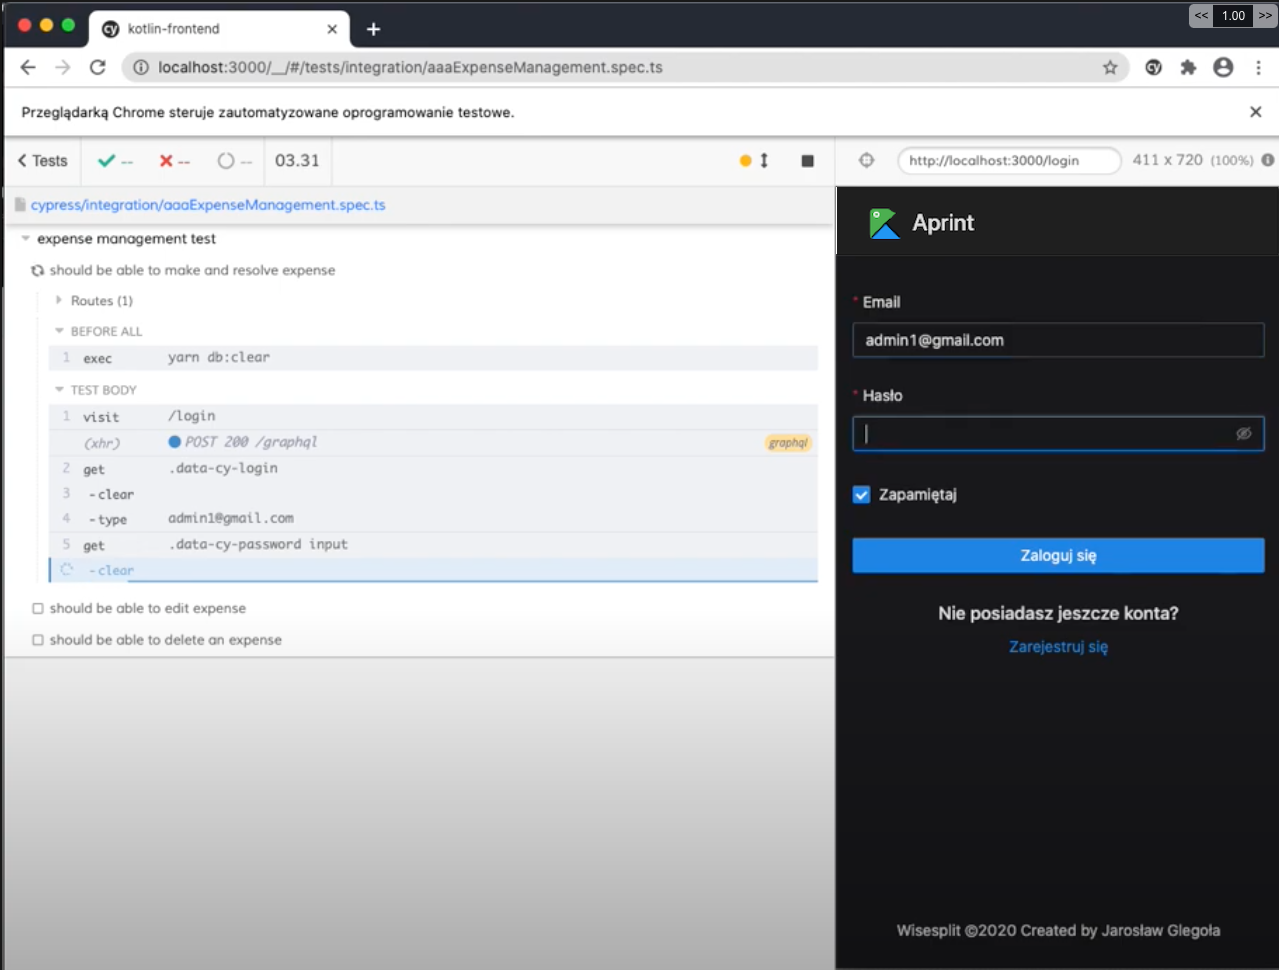
\includegraphics[width=\textwidth]{cypress-imape.png}
    \caption{Panel Cypress.io} \label{fig-cypress}
\end{figure}

\subsection{Testy wizualnej regresji aplikacji klienckiej}
Testy wizualnej regresji zapewniają wizualną poprawność interfejsu użytkownika. Dzięki nim mogłem programowo symulować sytuacje biznesowe, a następnie przy pomocy biblioteki Cypress.io robić zrzuty ekranu. Testy wizualnej regresji działają podobnie jak testy migawkowe, tylko zamiast zapamiętywania wartości zwróconej przez funkcję Cypress zapamiętuje zrzut ekranu przeglądarki. Gdy pierwszy zrzut ekranu aplikacji został zrobiony podczas pierwszego uruchomienia testu, każde następne uruchomienie tego samego testu będzie robiło kolejny zrzut, a następnie porównywało z poprzednim. W taki sposób możemy sprawdzać, czy po zmianach w kodzie nie nastąpiła niepożądana zmiana w wyglądzie aplikacji. Jeżeli takie dwa zrzuty się różnią, test wyświetli komunikat błędu a następnie wyświetli różniące się zrzuty ekranu i wyróżni wszystkie różniące się piksele obu zdjęć. Jeżeli natomiast zmiana wyglądu była zamierzona, programista może zaakceptować zmiany w teście i od tego momentu w następnych testach porównywać z nowym wyglądem.

% todo change screen to have new name and logo
\begin{figure}
    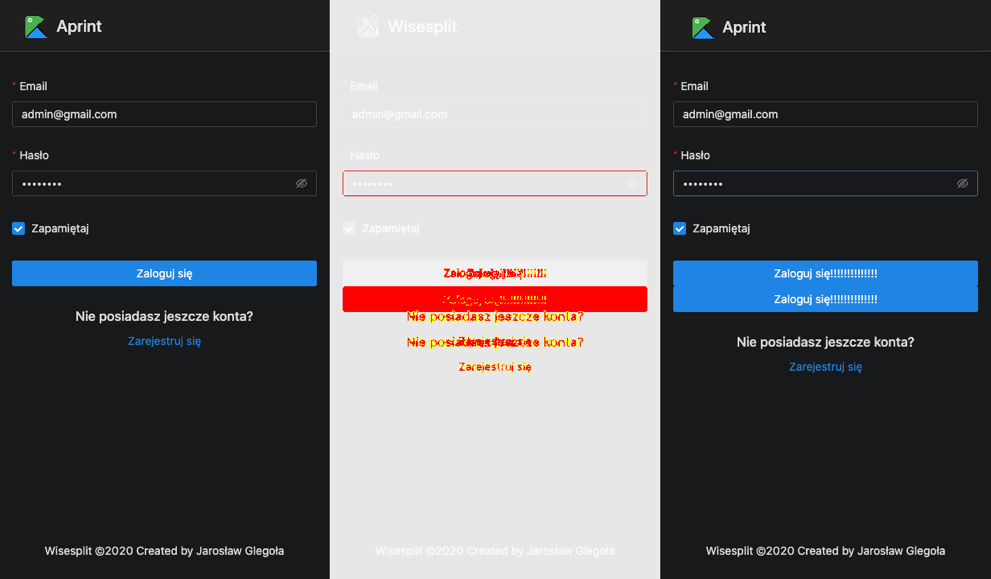
\includegraphics[width=\textwidth]{wisual-regression.png}
    \caption{Przykład wyniku nieudanego testu wizualnej regresji} \label{fig-cypress-vr}
\end{figure}


\subsection{Testy integracyjne aplikacji serwerowej}
Aplikację serwerową testowałem głównie integracyjnie. Do pisania testów wybrałem język Groovy i bibliotekę Spock w środowisku JUnit. Testy integracyjne serwera nie różnią się w dużej mierze od testów integracyjnych aplikacji klienckiej. Jedyną różnicą jest to, że nie posiadamy wizualnej części. Testy integracyjne testują wszystkie elementy aplikacji serwerowej: zapytania klienckie, logikę biznesową oraz integrację z bazą danych.
         % Wygodnie jest trzymać każdy rozdział w osobnym pliku.
\newpage
\section{Prezentacja aplikacji}
W tym rozdziale zostaną przedstawione poszczególne ekrany występujące w aplikacji w różnych stanach. Do poszczególnych sekcji będą też podane wymagania, które dane ekrany spełniają. W każdym podrozdziale zaprezentuję jeden ekran aplikacji.
 

Aplikacja została stworzona w stylu ciemnym, zgodnie ze wymaganiami specyfikacją Ant Design. Przykłady zostaną zaprezentowane w wersji na telefony, komórkowe, lecz aplikacja działa poprawnie z ekranami tabletów oraz większych ekranów komputerów i laptopów.

\clearpage
\subsection{Ekran logowania}
Ekran logowania jest połączony z ekranem rejestracji. Na ekranie widnieje przycisk \emph{Zarejestruj się}, który po kliknięciu sprawia, że pojawiają się dwie dodatkowe kontrolki do wprowadzania tekstu, gdzie użytkownik musi powtórzyć hasło i podać imię i nazwisko, które nie są wymagane przy formularzu logowania. W kroku rejestracji widnieje przycisk \emph{Zaloguj się}, który ukrywa te dwie kontrolki. Zmiana pomiędzy logowaniem a rejestracją nie powodują utraty danych zawartych w elementach. Po poprawnym wypełnieniu formularza użytkownik zostaje przekierowany na ekran listy wydatków. Ekran spełnia wymagania WF1 oraz WF2.


\begin{figure}[h!]%
    \centering
    \subfloat[\centering Krok logowania]{{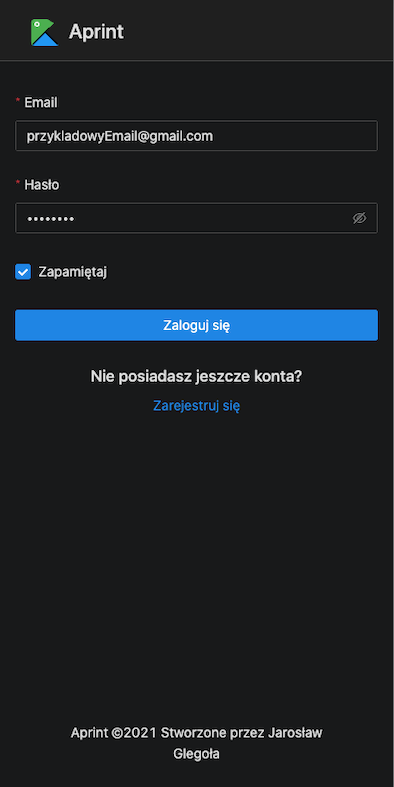
\includegraphics[width=0.45\textwidth]{presentation/login-login.png} }}%
    \qquad
    \subfloat[\centering Krok rejestracji]{{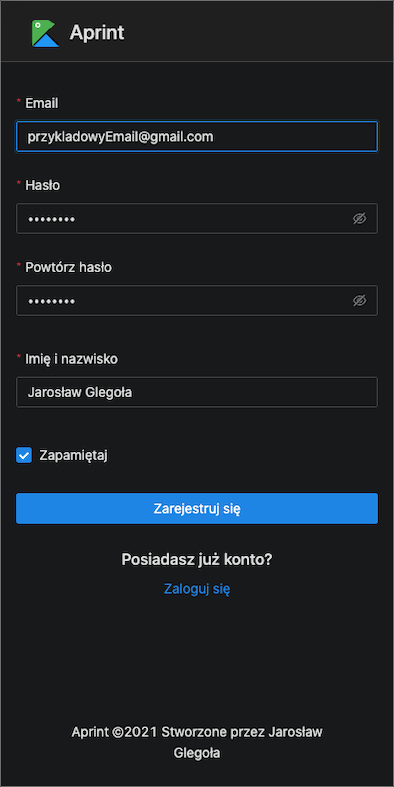
\includegraphics[width=0.45\textwidth]{presentation/login-register.png} }}%
    \caption{Ekran logowania i rejestracji}%
\end{figure}

\clearpage
\subsection{Wydatki}
\subsubsection{Ekran listy wydatków}
Na tym ekranie użytkownik ma dostęp do listy wszystkich wydatków w których uczestniczy. Na górze ekranu widzimy całkowity bilans kwoty którą powinien zapłacić oraz kwotę, którą powinien otrzymać od innych użytkowników oraz całkowity bilans tych dwóch kwot. Te dwa kafelki są interaktywne i kliknięcie na jeden z nich zmienia listę wydatków. Ta część odpowiada za wymaganie WF10.

Jeżeli zaznaczona jest opcja \emph{Inni są tobie winni}, na liście wydatków pojawiają się wydatki, które założył dany użytkownik, a po zmianie na opcję \emph{Ty jesteś winny w sumie} pojawiają się na liście wydatki, w których użytkownik uczestniczy. Domyślnie ukazane są nieukończone wydatki, ale użytkownik ma możliwość zaznaczenia opcji \emph{Pokaż zakończone}, która pokazuje wszystkie wydatki włączając w to te zakończone.

\begin{figure}[h]%
    \centering
    \subfloat{{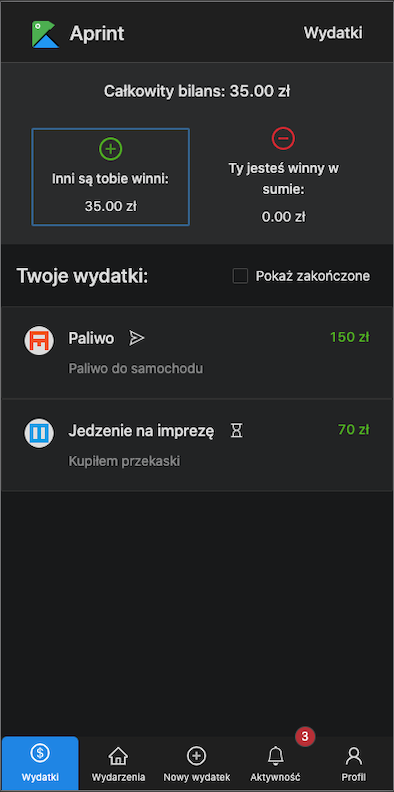
\includegraphics[width=0.45\textwidth]{presentation/responsive-sm.png} }}%
    \caption{Ekran listy wydatków}%
\end{figure}

\clearpage
\subsubsection{Ekran wydatku}
Na ekranie wydatku są ukazane dane jednego wydatku. Na ekranie jest też pokazany aktualny stan wydatku na komponencie zwanym \emph{krokami}. Dzięki temu komponentowi stan wydatku jest bardziej zrozumiały dla użytkownika. Dodatkowo są też ukazani uczestnicy oraz wszystkie płatności stworzone w ramach wydatku. Inicjator wydatku może z tego poziomu zarządzać wydatkiem, czyli akceptować płatności oraz może zakończyć wydatek. Z tego poziomu może też przejść do ekranu formularza edycji wydatku.

\begin{figure}[h!]%
    \centering
    \subfloat[\centering Wydatek oczekujący]{{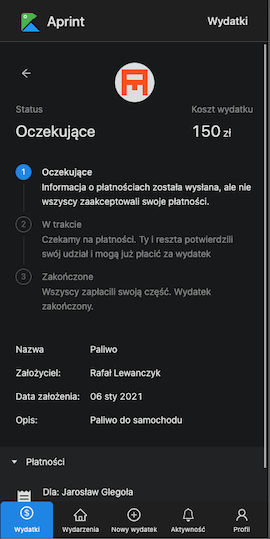
\includegraphics[width=0.31\textwidth]{presentation/expense-waiting.png} }}%
    \qquad
    \subfloat[\centering Wydatek w trakcie]{{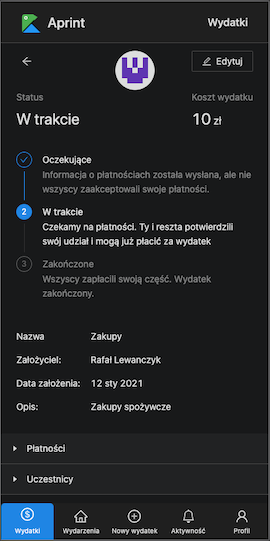
\includegraphics[width=0.31\textwidth]{presentation/expense-in-progress.png} }}%
    \qquad
    \subfloat[\centering Wydatek zakończona]{{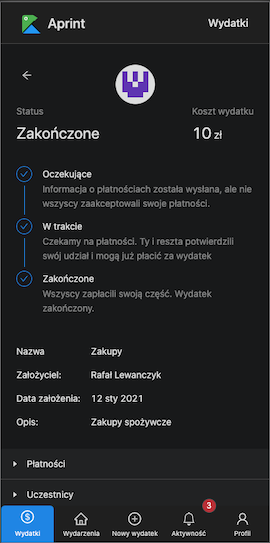
\includegraphics[width=0.31\textwidth]{presentation/expense-ended.png} }}%
    \qquad
    \subfloat[\centering Widok płatności i uczestników wydatku]{{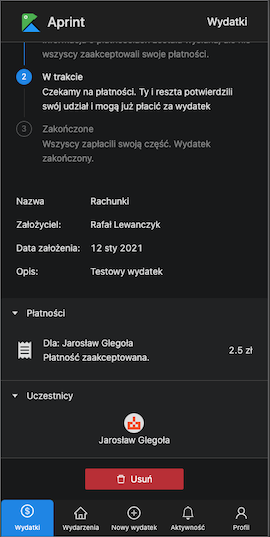
\includegraphics[width=0.31\textwidth]{presentation/expense-bottom-view.png} }}%
    \caption{Ekrany wydatku}%
\end{figure}

\clearpage
\subsubsection{Formularz wydatku}
Ekran tworzenia wydatku pozwala na tworzenie nowych wydatków oraz ich edycji. Wydatki możemy tworzyć dla wydarzeń, grup lub wybierając tylko znajomych. Dane dla każdego typu wydatku się różnią, więc formularz będzie wyglądał inaczej dla każdego typu. Ten formularz spełnia wymaganie WF4 oraz WF7.


\begin{figure}[h!]%
    \centering
    \subfloat[\centering Płatność niepotwierdzona]{{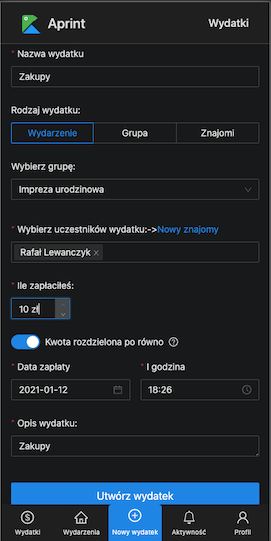
\includegraphics[width=0.31\textwidth]{presentation/expense-form-event.png} }}%
    \qquad
    \subfloat[\centering Potwierdzanie płatności]{{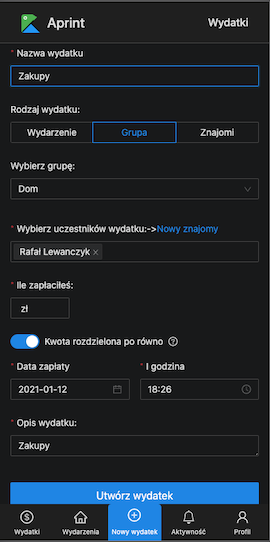
\includegraphics[width=0.31\textwidth]{presentation/expense-form-group.png} }}%
    \qquad
    \subfloat[\centering Płatność potwierdzona]{{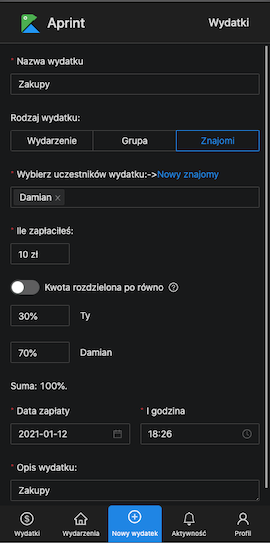
\includegraphics[width=0.31\textwidth]{presentation/expense-form-friends.png} }}%
    \caption{Formularz wydatku}%
\end{figure}

\clearpage
\subsection{Ekran płatności}
Gdy użytkownik zostanie zaproszony do wydatku tworzony zostaje dla niego obiekt płatności, który jest przedstawiony na ekranie płatności. Na tym ekranie są zawarte informacje wydatku do którego należy płatność oraz informacje o samej płatności. Z poziomu tego ekranu użytkownik może też zarządzać stanem swojej płatności, czyli akceptować płatność, potwierdzać wpłatę lub odrzucać płatność. Ekran spełnia wymaganie WF5.

\begin{figure}[h!]%
    \centering
    \subfloat[\centering Płatność niepotwierdzona]{{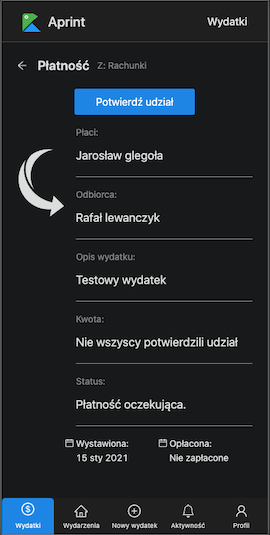
\includegraphics[width=0.31\textwidth]{presentation/payment-to-confirm.png} }}%
    \qquad
    \subfloat[\centering Potwierdzanie płatności]{{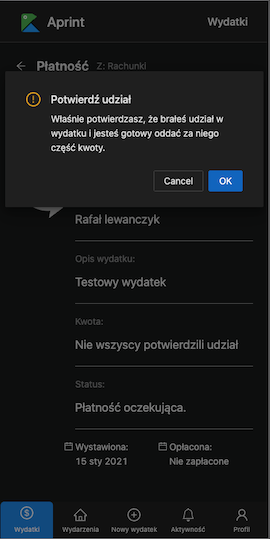
\includegraphics[width=0.31\textwidth]{presentation/payment-confirmation.png} }}%
    \qquad
    \subfloat[\centering Płatność potwierdzona]{{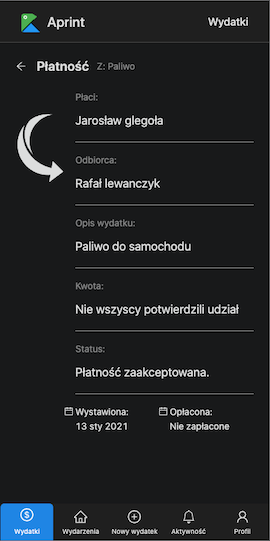
\includegraphics[width=0.31\textwidth]{presentation/payment-confirmed.png} }}%
    \qquad
    \subfloat[\centering Płatność gotowa do zapłaty]{{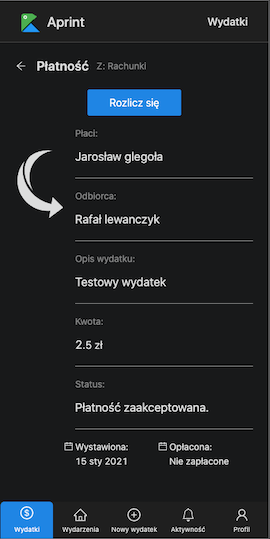
\includegraphics[width=0.31\textwidth]{presentation/payment-to-pay.png} }}%
    \caption{Ekran płatności}%
\end{figure}

\clearpage
\subsection{Ekran wydarzeń, grup i grup znajomych}
\subsubsection{Listy wydarzeń, grup i grup znajomych}
Na głównym ekranie list znajdują się zakładki, dzięki którym użytkownik może wybrać ich typ. Na tym ekranie mogą pojawić się listy wydarzeń, grup, grup znajomych i zaproszeń. Po kliknięciu na każdy element listy możemy przejść na ekran pojedynczego elementu.

\begin{figure}[h!]%
    \centering
    \subfloat[\centering Lista wydarzeń]{{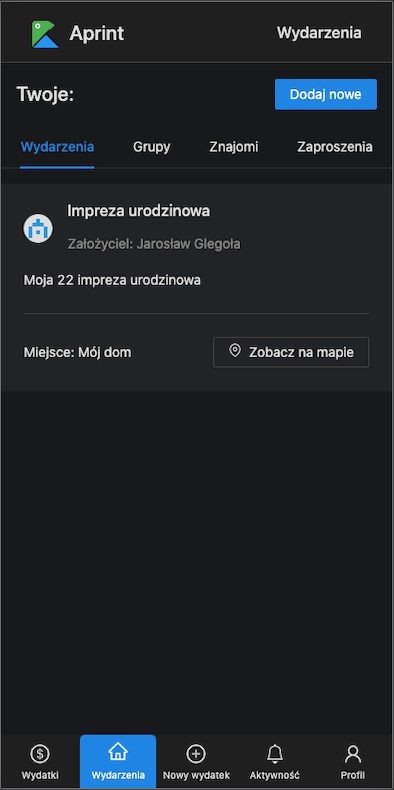
\includegraphics[width=0.45\textwidth]{presentation/event-event-list.png} }}%
    \qquad
    \subfloat[\centering Lista grup]{{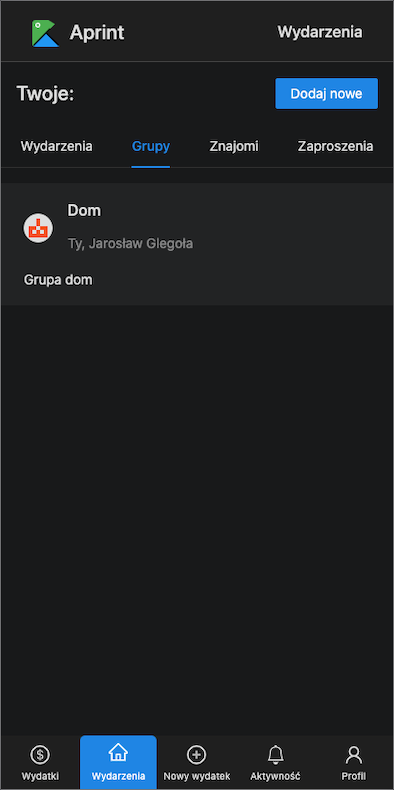
\includegraphics[width=0.45\textwidth]{presentation/event-group-list.png} }}%
    \caption{Listy wydarzeń i grup}%
\end{figure}

\clearpage
\subsubsection{Ekrany wydarzeń, grup i grup znajomych}
Poniżej ukazane są zrzuty ekranu widoków pojedynczych wydarzeń i grup. Na tym widoku są ukazane informacje na temat elementu, lista wydatków oraz wszyscy uczestnicy. Użytkownik z tego poziomu może dołączyć do elementu klikając przycisk \emph{wezmę udział}, gdy użytkownik jeszcze nie zaakceptował zaproszenia, lub opuścić wydarzenie klikając ten sam przycisk, gdy zaproszenie już zaakceptował. Ekran spełnia wymaganie WF6.

Inicjator z tego poziomu może dodawać nowych uczestników, usuwać użytkowników z elementu oraz usuwać dany element.

\begin{figure}[h!]%
    \centering
    \subfloat[\centering Ekran wydarzenia]{{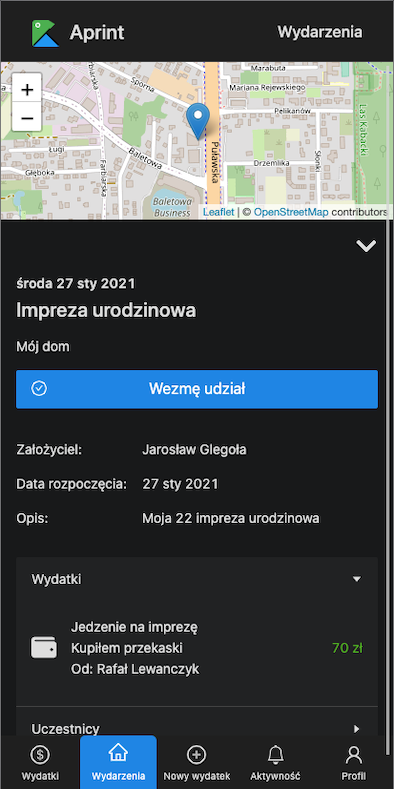
\includegraphics[width=0.45\textwidth]{presentation/event-event-view.png} }}%
    \qquad
    \subfloat[\centering Ekran grupy]{{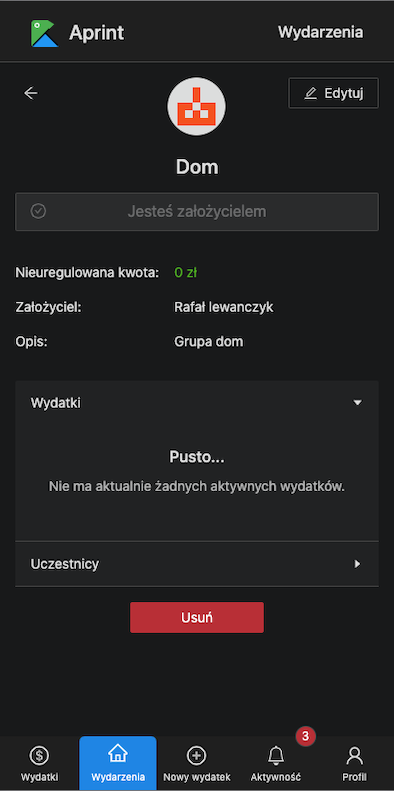
\includegraphics[width=0.45\textwidth]{presentation/event-group-view.png} }}%
    \caption{Ekrany wydarzeń i grup}%
\end{figure}

\clearpage
\subsubsection{Formularz dodawania elementu}
Formularz dodawania elementu umożliwia dodawanie nowego elementu oraz edycję już utworzonego elementu. Formularz może być wyświetlany w dwóch trybach: \emph{Wydarzenie} oraz \emph{Grupa}. W trybie \emph{wydarzenie} mamy możliwość dodania wydarzenia dodatkowo posiadającego datę rozpoczęcia, miejsca wydarzenia oraz możliwości wyboru miejsca na mapie. W trybie \emph{Grupa} mamy możliwość dodania tylko nazwy uczestników i opisu.

\begin{figure}[h!]%
    \centering
    \subfloat{{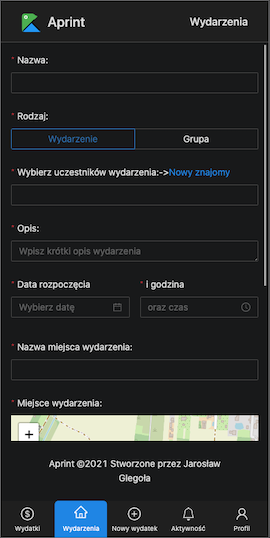
\includegraphics[width=0.31\textwidth]{presentation/event-form-p1.png} }}%
    \qquad
    \subfloat{{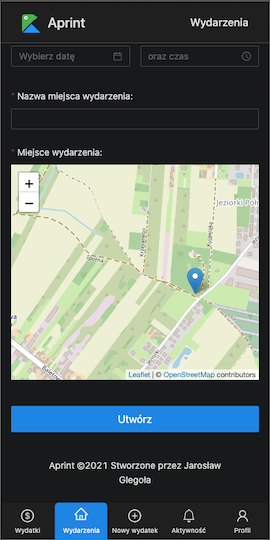
\includegraphics[width=0.31\textwidth]{presentation/event-form-p2.png} }}%
    \caption{Formularz w trybie typu \emph{Wydarzenie}}%
\end{figure}

\begin{figure}[h!]%
    \centering
    \subfloat{{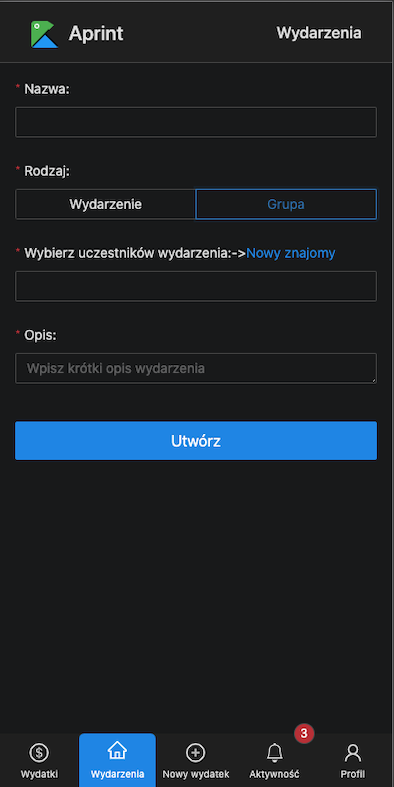
\includegraphics[width=0.45\textwidth]{presentation/event-group-form.png} }}%
    \caption{Formularz w trybie typu \emph{Grupa}}
\end{figure}

\clearpage
\subsection{Aktywność}
Panel aktywności wyświetla użytkownikowi wszystkie dostępne powiadomienia w formie listy. Po kliknięciu w elementy aplikacja przekierowywuje użytkownika do odpowiednich stron np. po kliknięciu w pierwszy element ukazany na rysunku ~\ref{fig:notificationList} zostaniemy przekierowywani do wydatku do którego użytkownik został dołączony. Dodatkowo, gdy są na ekranie nowe powiadomienia wyświetlają się przy nich czerwone kropki, aby zwrócić na nie uwagę użytkownika (przykład na rysunku ~\ref{fig:notificationListNew}). Każde powiadomienie może być usunięte przez użytkownika. Powiadomienia są posortowane w taki sposób, aby najnowsze pojawiały się na samej górze ekranu. Ekran spełnia wymaganie WF8.

\begin{figure}[h!]%
    \centering
    \subfloat[\centering Lista aktywności]{{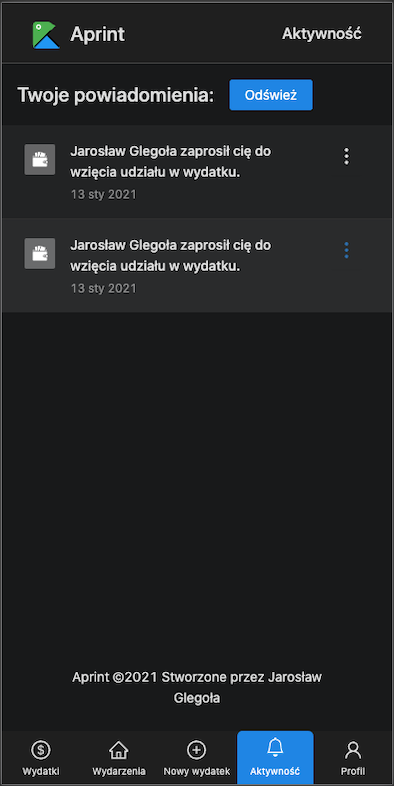
\includegraphics[width=0.45\textwidth]{presentation/notification-list.png} \label{fig:notificationList} }}%
    \qquad
    \subfloat[\centering Lista aktywności z nowym powiadomieniem]{{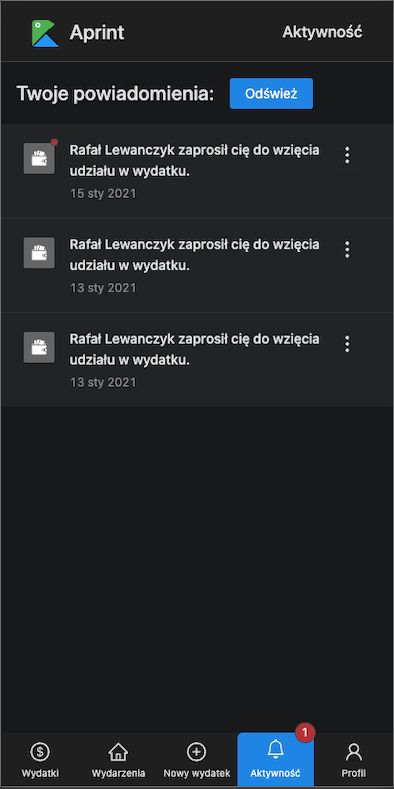
\includegraphics[width=0.45\textwidth]{presentation/notification-list-new.png} \label{fig:notificationListNew}}}%
    \caption{Ekran listy powiadomień}%
\end{figure}

\clearpage
\subsection{Ekrany użytkownika}
\subsubsection{Ekran informacji o użytkowniku}
Na ekranie użytkownika są wyświetlone dane użytkownika tj. imię, numer konta, email. Z poziomu tego ekranu użytkownik może edytować te informacje oraz wylogować się z konta.

\begin{figure}[h!]%
    \centering
    \subfloat[\centering Informacje użytkownika]{{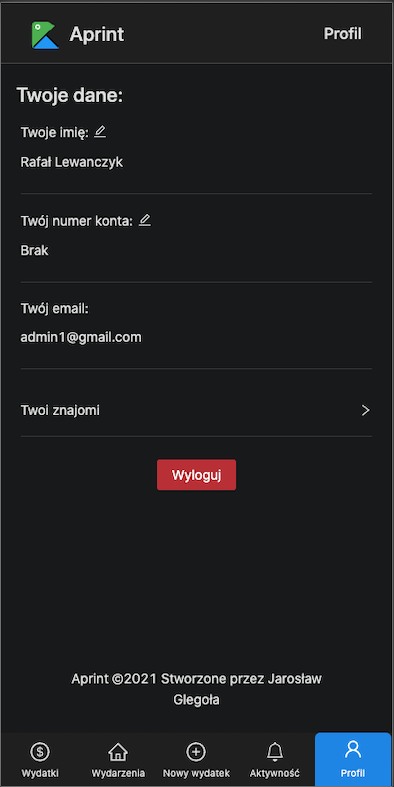
\includegraphics[width=0.45\textwidth]{presentation/user-profile.png} }}%
    \qquad
    \subfloat[\centering Edycja numeru konta]{{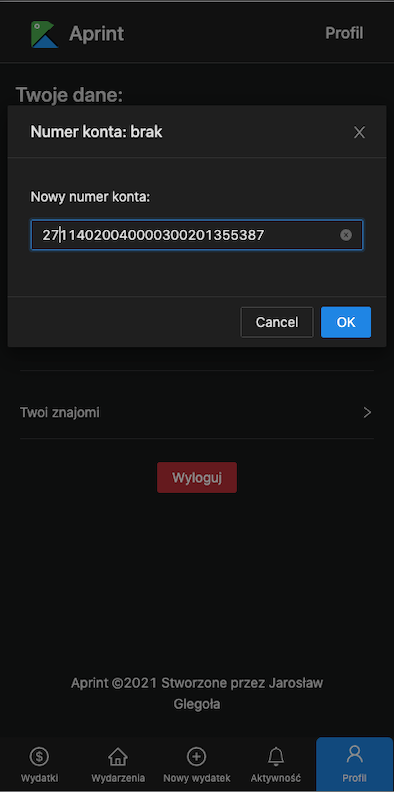
\includegraphics[width=0.45\textwidth]{presentation/user-change-number.png}}}%
    \caption{Ekran użytkownika}%
\end{figure}

\clearpage
\subsubsection{Ekran znajomych}
Na ekranie znajomych znajduje się lista wszystkich znajomych użytkownika oraz mechanizm dodawania nowych użytkowników. Dodatkowo z tego poziomu użytkownik może też usuwać innych użytkowników z listy swoich znajomych. Ekran spełnia wymaganie WF3.

\begin{figure}[h!]%
    \centering
    \subfloat[\centering Lista znajomych]{{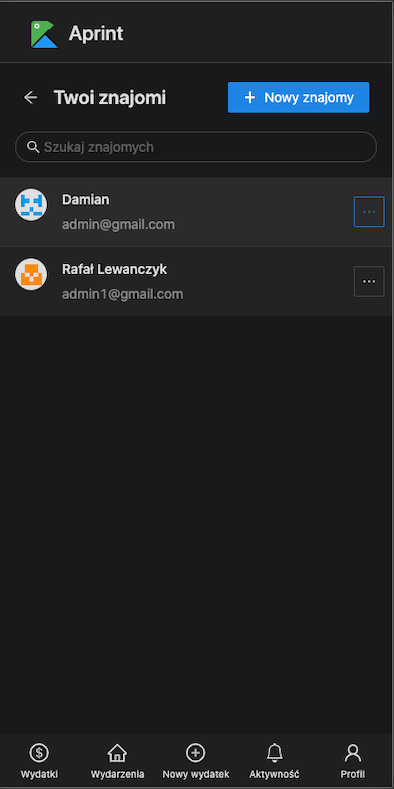
\includegraphics[width=0.45\textwidth]{presentation/friend-list.png} }}%
    \qquad
    \subfloat[\centering Dialog dodawania nowych znajmych]{{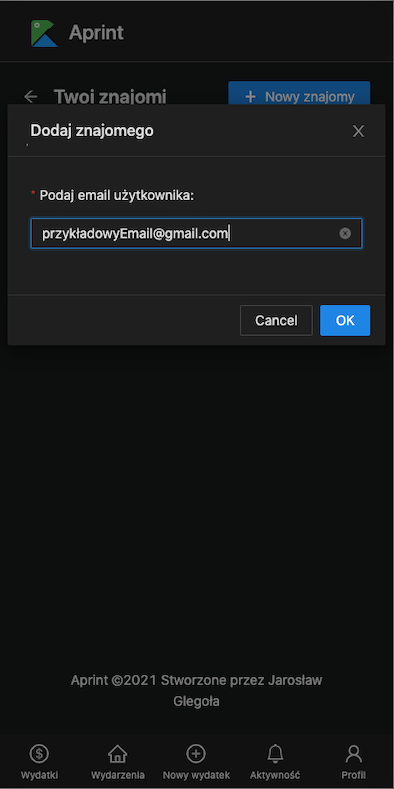
\includegraphics[width=0.45\textwidth]{presentation/friend-add.png}}}%
    \caption{Ekran znajomych}%
\end{figure}

\clearpage
\subsubsection{Ekran innego użytkownika}
Użytkownik może też zobaczyć informacje o innym użytkowniku: jego email, imie oraz numer konta na który może przelać pieniądze za płatność. Na tym ekranie dostępne są też informacje o balansie pieniężnym pomiędzy użytkownikami. Ekran spełnia wymaganie WF11.

\begin{figure}[h!]%
    \centering
    \subfloat[\centering Lista znajomych]{{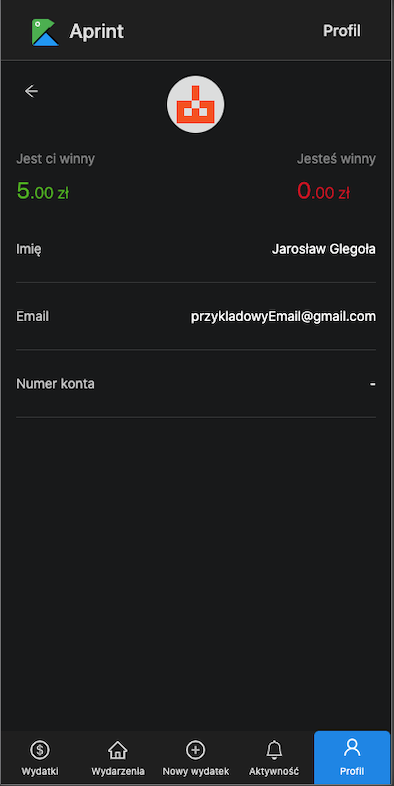
\includegraphics[width=0.45\textwidth]{presentation/friend-view.png} }}%
\end{figure}
         % Wygodnie jest trzymać każdy rozdział w osobnym pliku.
                            % na nowe wersje, a cały tekst pracy pozostaje nienaruszony.

\newpage % Rozdziały zaczynamy od nowej strony
\section{Summatio}          % Można też pisać rozdziały w jednym pliku.
\lipsum[5-10]

%--------------------------------------------
% Literatura
%--------------------------------------------
\cleardoublepage % Zaczynamy od nieparzystej strony
\printbibliography

%--------------------------------------------
% Spisy (opcjonalne)
%--------------------------------------------
\newpage
\pagestyle{plain}

% Wykaz symboli i skrótów.
% Pamiętaj, żeby posortować symbole alfabetycznie
% we własnym zakresie. Ponieważ mało kto używa takiego wykazu,
% uznałem, że robienie automatycznie sortowanej listy
% na poziomie LaTeXa to za duży overkill.
% Makro \acronymlist generuje właściwy tytuł sekcji,
% w zależności od języka.
% Makro \acronym dodaje skrót/symbol do listy,
% zapewniając podstawowe formatowanie.
% //AB
\vspace{0.8cm}
\acronymlist
\acronym{EiTI}{Wydział Elektroniki i Technik Informacyjnych}
\acronym{PW}{Politechnika Warszawska}
\acronym{WEIRD}{ang. \emph{Western, Educated, Industrialized, Rich and Democratic}}

\listoffigurestoc     % Spis rysunków.
\vspace{1cm}          % vertical space
\listoftablestoc      % Spis tabel.
\vspace{1cm}          % vertical space
\listofappendicestoc  % Spis załączników

% Załączniki
\newpage
\appendix{Nazwa załącznika 1}
\lipsum[1-8]

\newpage
\appendix{Nazwa załącznika 2}
\lipsum[1-4]

% Używając powyższych spisów jako szablonu,
% możesz tu dodać swój własny wykaz bądź listę,
% np. spis algorytmów.

\end{document} % Dobranoc.
